\chapter{模板简介}
%
与很多外文杂志社不同,大部分中文期刊都不提供\LaTeX{}模板给投稿者使用,也很少有学校给学生提供官方的毕业论文模板。目前github上的大部分模板都是由学生发起的非官方模板。在此感谢Shun Xu以及yecfly等人的工作,他们的无私贡献使得华南理工大学硕博士毕业论文也可以使用\LaTeX{}撰写。

本模板是直接修改前人的模板得到的,更详细的介绍可到\parencite{_,_a}下载。本章仅从用户的角度简要介绍模板的使用,而尽量避免涉及\LaTeX{}的模板制作细节(实际上是因为本人也不会)。正如我们使用手机并不需要了解麦克斯韦方程组,使用\LaTeX{}写作也无需了解模板是如何制作的。

\LaTeX{}的源代码保存在后缀名为.tex的文件中。当编写长篇文档时,例如当编写书籍、毕业论文时,单个源文件会使修改、校对变得十分困
难。将源文件分割成若干个文件,例如将每章内容单独写在一个文件中,会大大简化修改和校对
的工作。为方便,本文将scutthesis.tex文件称为主文件,而将abstract.tex、chapter0x.tex、conclusion.tex等文件称为章节文件。

值得注意的是,要每次编译时都更新参考文献著录,TeXstudio软件的选项->设置中的构建并查看、编译器需要设置成如图\ref{TeXstudio}、\ref{setup}所示。此时只需在任意一个文件中点击构建并查看按钮即可编译文档。每次编译都更新参考文献会使得编译时间很长。
\begin{figure}[htbp]
	\centering
	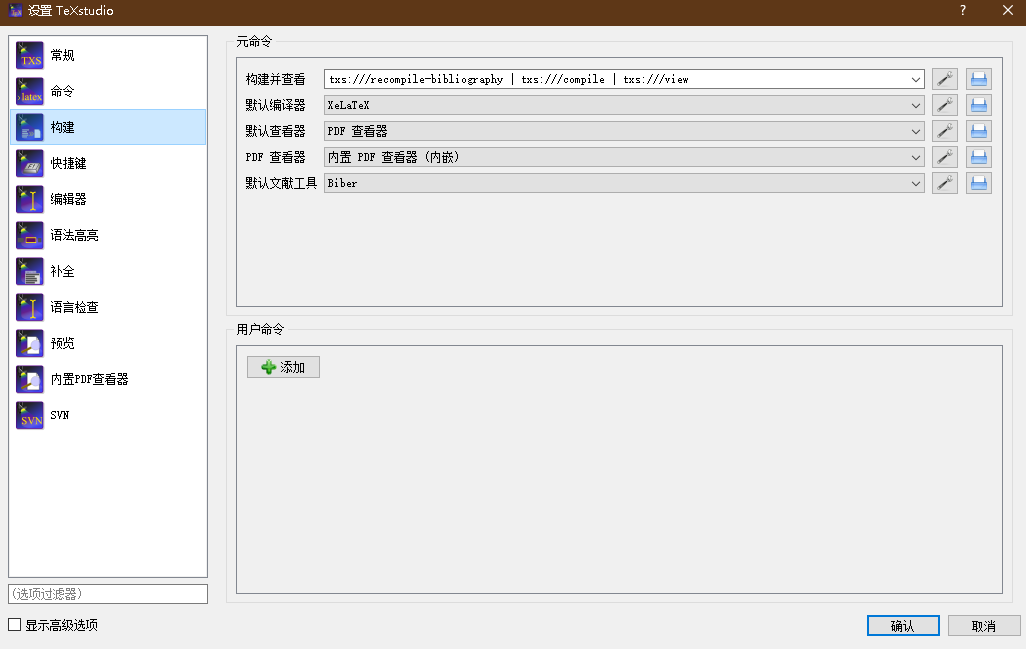
\includegraphics[scale=0.55]{Fig/TeXstudio.png}
	\caption{\label{TeXstudio}TeXstudio环境}
\end{figure}
\begin{figure}[htbp]
	\centering
	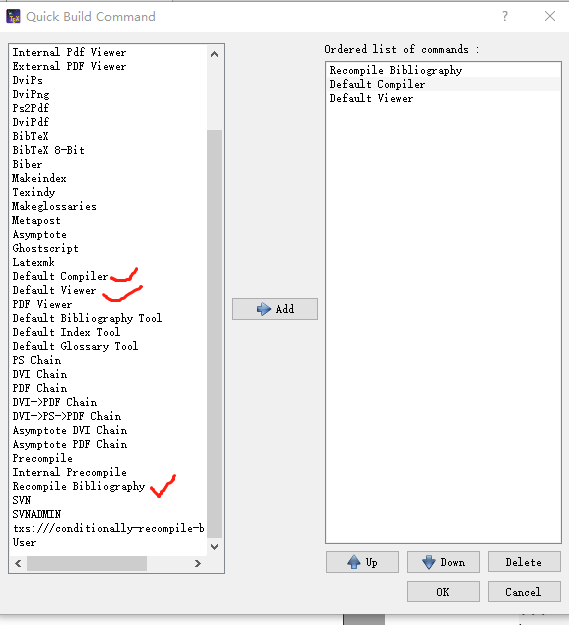
\includegraphics[scale=0.55]{Fig/setup.png}
	\caption{\label{setup}TeXstudio编译选项}
\end{figure}

\section{主文件}
scutthesis.tex文件相当于主函数,调用各章的内容。\LaTeX{}源代码以一个\textbackslash{}documentclass 命令作为开头,它指定了文档使用的文档类。文档类规定了\LaTeX{}源代码所要生成的文档的性质——普通文章、书籍、演示文稿、个人简
历等等。
\begin{lstlisting}
\documentclass[⟨options⟩]{⟨class-name⟩}
\end{lstlisting}
其中class-name为文档类的名称,如\LaTeX{}提供的article, book, report,可在其基础上派
生的一些文档类或者有其它功能的一些文档类。\LaTeX{}提供的基础文档类见文献\parencite{_c}。还可以自定义文档类,如华南理工大学硕博士论文文档类scutthesis,其实现保存在后缀名为.cls的文件中。可选参数options 为文档类指定选项。


document环境当中的内容是文档正文:
\begin{lstlisting}
\begin{document}
正文内容
\end{document}
\end{lstlisting}
正文中包含各章节内容:
\begin{lstlisting}
\chapter{摘\texorpdfstring{\quad}{}要}

垂直领域对话生成技术是构建智能对话系统中重要的基础技术,该技术旨在为用户解决特定领域的问题、提供专业解答。目前该技术已经广泛应用在医疗保健、金融、法律、科技等领域的服务助手、答疑机器人等应用中,具有很高的研究价值。

目前主流的面向垂直领域的对话生成方法,都是基于检索增强的自回归模型设计的。然而,现有面向垂直领域的检索增强对话生成存在以下难点:1)专有领域背景知识丰富,且逻辑相对复杂;2)用户问题形式多样,意图难以理解。针对以上存在的两个问题,本文采取的研究方案如下:

\begin{enumerate}[topsep = 0 pt, itemsep= 0 pt, parsep=0pt, partopsep=0pt, leftmargin=0pt, itemindent=44pt, labelsep=6pt, listparindent=24pt, label=\arabic*)]
	\item 针对专有领域背景知识丰富、逻辑相对复杂的问题,提出了基于内外部知识对齐的检索增强对话生成方法。该方法利用一个语义切分模块提取知识文档的文档级信息和实体级信息,并将提取出来的知识分别用于构建外部知识库和内部知识注入,实现垂直领域对话模型内外部知识对齐。本文将该方法应用于金融分析领域,在真实股票价格预测任务和金融问答任务上验证了该方法的有效性。

	\item 针对用户问题形式多样、意图难理解的问题,提出了基于人类偏好对齐的检索增强对话生成方法。该方法通过采集人类对真实场景对话样本的偏好,利用大型语言模型的理解与分析能力进行问题优化,并训练单独的问题优化语言模型,实现了与模型无关的、可解释、效果稳定的人类偏好对齐。本文分别在两个不同的基准测试机上与目前主流的语言模型对齐方法进行实验比较,证明了该方法能同时提升知识文档召回准确率和模型理解与用户意图的一致性。
\end{enumerate}

\keywordsCN{对话系统;人类偏好对齐;检索增强生成;自回归语言模型}

\chapter{Abstract}

Vertical domain dialog generation technology is an important basic technology in building intelligent dialog system, which aims to solve problems in specific fields and provide professional answers for users. At present, the technology has been widely used in the fields of health care, finance, law, science and technology and other service assistants, answering robots and other applications, has high research value.

At present, the mainstream vertical-domain oriented dialogue generation methods are all designed based on retrieve-enhanced autoregressive models. However, there are the following difficulties in the current vertic-domain-oriented retrieval enhanced dialogue generation: 1) the background knowledge of the proprietary domain is rich, and the logic is relatively complex; 2) User questions come in many forms and their intentions are hard to understand. In view of the above two problems, the research plan adopted in this paper is as follows:

\begin{enumerate}[topsep = 0 pt, itemsep= 0 pt, parsep=0pt, partopsep=0pt, leftmargin=0pt, itemindent=44pt, labelsep=6pt, listparindent=24pt, label=\arabic*)]
	\item Aiming at the problem of rich background knowledge and relatively complex logic in proprietary domain, a search enhanced dialogue generation method based on internal and external knowledge alignment is proposed. In this method, a semantic segmentation module is used to extract document-level information and entity-level information from knowledge documents, and the extracted knowledge is used to construct external knowledge base and internal knowledge injection respectively, so as to realize internal and external knowledge alignment in vertical domain dialogue model. In this paper, the method is applied to financial analysis, and the validity of the method is verified on real stock price prediction task and financial question answering task.

	\item Aiming at the problem of various forms of user questions and difficult to understand the intention, a search enhancement dialog generation method based on human preference alignment is proposed. By collecting human preferences for real scene dialogue samples, the method uses the understanding and analysis ability of large-scale language models to optimize the problem, and trains a single problem optimization language model, and realizes the model-independent, interpretable and stable human preference alignment. In this paper, two different benchmarking machines are used to compare with the current mainstream language model alignment methods, and it is proved that this method can improve the accuracy of knowledge document recall and the consistency of model understanding and user intention.
\end{enumerate}

\keywordsEN{Dialogue System; Human Preference Alignment; Retrieval Augmented Generation; Regressive Language Model} % 中英文摘要
\tableofcontents	% 目录
\listoftables	% 表格目录(可选)
\listoffigures	% 插图目录(可选)
\chapter{主要符号对照表}
【本节论文规范为可选,如果你的论文没有相关内容那么去除这一节;如果有,则删除这一行注释。】
\begin{table}
	\centering{}%
	\begin{tabular}{l>{\centering}p{0.5cm}l}
	 $ \bm{X}_n\bm{Y}_n\bm{Z}_n $-地理坐标系           &  & ${\bm{X}_b}{\bm{Y}_b}{\bm{Z}_b}$-机体坐标系\tabularnewline
	 $ \psi $-偏航角								   &  & $\theta$-俯仰角\tabularnewline
	 $\varphi$-滚转角  							   &  & $\bm{R}^n_b$、$\bm{R}$-机体系到NED系的旋转矩阵\tabularnewline
	 $\bm{G}$-NED系的重力  							  &  &   $\varphi_0 $-气动面安装角\tabularnewline
	 $ w $-系统的外部扰动								&  &  $T$-系统采样周期\tabularnewline
	 $\bm{F}$-机体系的气动力 						    &  &   $\bm{M}$-机体系的气动力矩\tabularnewline
	 $\rho$-空气密度 								  &  &  $C_{D,x} $、$ C_{D,y} $、$ C_{D,z} $-沿机体轴阻力系数\tabularnewline
	 $A_x $、$ A_y $、$ A_z $-沿机体轴的截面面积 		 &  &  $v$-机身相对于空气的速度分量\tabularnewline 
	 $l_{a}$-机身气动阻力作用点与重心的距离   			  &  &  $V_c$-气体在无穷远处的速度\tabularnewline
	 $T_d$-涵道体升力  								 &  &  $T_p$-风扇升力\tabularnewline
	 $T_a$-总升力 								      &  &  $q_a$-涵道升力分配系数\tabularnewline
	 $ p_U $-桨盘上表面压强 						   &  &  $p_L$-桨盘下表面压强\tabularnewline
	 $V_c+V_i$-桨盘上下表面气体速度 					 &  &  $S$-桨盘面积\tabularnewline
	 $ V_i $-桨盘处气流诱导速度 						  &  &  $ V_{cr} $-理想自转下降速率\tabularnewline
	 $ Q $-风扇扭矩 								 &  &  $ \varpi $-风扇转速\tabularnewline
	 $\mu$-环绕涵道角度变量 						  &  &  $\hat{\bm{i}}$-沿机体系$x$轴方向的单位矢量\tabularnewline 
	 $\hat{\bm{j}}$-沿机体系$y$轴方向的单位矢量  	   &  &  $C_{l, d}(\alpha_d)$-涵道翼型升力曲线\tabularnewline 
	 $C_{d, d}(\alpha_d)$涵道翼型阻力曲线  		      &  &  $c_d$-涵道翼型弦长\tabularnewline 
	 $C_{l_{\alpha}}$-风管翼型升力曲线斜率  			 &  &  $C_{l, \min }$、$ C_{l, \max } $-升力系数极限\tabularnewline 
	 $C_{d, o }$、$C_{d, g }$-拟合阻力曲线经验常数 	&  &  $R$-风扇半径\tabularnewline 
	 $C_{d u c t}$ - 常值比例系数  					&  &  $l_{d}$-重心与涵道气动力作用点的距离\tabularnewline
	 $k_{\delta}$-操纵面气动升力系数 				 &  &  $\alpha_d$-攻角\tabularnewline
	 $ I_{b}$-风扇转动惯量  						   &  &  $ d_{af} $ 、$ d_{ds} $-风扇扭矩常系数\tabularnewline
	 $\bm{L}_{{r}}$-风扇角动量  						&  & \tabularnewline 					
	\end{tabular}
\end{table}	% 符号对照表(可选)
\chapter{英文缩略词}
【本节论文规范为可选,如果你的论文没有相关内容那么去除这一节;如果有,则删除这一行注释。】
\begin{table}
	\centering{}%
	\begin{tabular}{ccc}
		SCUT  & South China University of Technology & 华南理工大学\tabularnewline
		&  & \tabularnewline
		&  & \tabularnewline
		&  & \tabularnewline
		&  & \tabularnewline
	\end{tabular}
\end{table} 	% 缩略词	
...
\chapter{绪论}
%
\section{研究背景和意义}
\subsection{研究背景和意义}
%
关于\LaTeX{}以及基于\LaTeX{}写作的好处不再赘述。\LaTeX{}的入门资料推荐文献\parencite{_g}以及文献\parencite{_c}。

这里主要是想推荐一种“学术生态”,即利用各种工具展开科研工作,以达到事半功倍的效果。需要用到以下软件:
\begin{enumerate}
	\item 	参考文献管理软件zotero\cite{_m}。很多人使用过endnote,但其实zotero也非常强大,强烈推荐。可到b站观看Struggle with Me出品的视频教程\cite{_k}入门。zotero不自带pdf阅读器,使用Adobe Acrobat pro DC即可。在Adobe中点击文件->属性->位置,即可打开文件所在位置,故亦不推荐更改zotero的文件系统。
	\item	可截图获取文献中公式的软件mathpix\cite{_h}。在阅读别人的论文时,很可能需要把文章中的公式抄下来放到自己的笔记中,方便以后组会报告甚至论文中使用,这时使用mathpix可直接截图获取\LaTeX{}源码,非常方便。该软件普通邮箱注册可每月50次免费,学校邮箱可100次,若信用卡注册可1000次。	
	\item	TeXstudio,相当于IDE。本模板是基于TeXstudio2020进行的,关于该软件的使用(快捷键等)可另行查找资料。编译时可以使用该软件,也可以运行文件目录的all.bat。TeXstudio的设置见第二章。
\end{enumerate}

本文的章节安排如下:

第一章,绪论。

第二章,模板简介。主要介绍各文件的内容。

第三章,常用环境。介绍论文写作中常用的环境,包括:图、表、公式、定理。基本涵盖了常用的命令。

%第三章,参考文献设置。本模板对旧版的改动主要是参考文献部分,本章将简单参考文献设置以及
%编译选项的设置等等。


	% 第一章
\chapter{相关研究现状}

人机对话系统一直是人工智能领域的重要研究方向,其旨在模拟人类并与人类形成连贯通顺的对话。本文所研究的面向垂直领域的对话生成是对话系统领域的其中一个下游任务,因此本章先对管道式对话系统和端到端式对话系统的研究进展和现状进行总结。然后,分别介绍面向垂直领域的对话生成和基于大型语言模型的对话生成的发展现状,并分析和总结其优点与不足。

\section{对话系统}

近年来,深度学习技术快速发展,促进了对话系统研究的发展\cite{JSJX201907001}。目前主流的对话系统实现方法从架构模式来看,可以分为管道式对话系统和端到端式对话系统。

\subsection{管道式对话系统}

图\ref{pipeline_dialogue_system}展示了管道式对话系统(Pipeline-based Dialogue System)结构的示意图,管道式对话系统主要包含四个模块:(1)自然语言理解(NLU)模块;(2)对话状态跟踪(DST)模块;(3)对话策略学习(PL)模块;(4)自然语言生成(NLG)模块。

\begin{figure}[htbp]
	\centering
	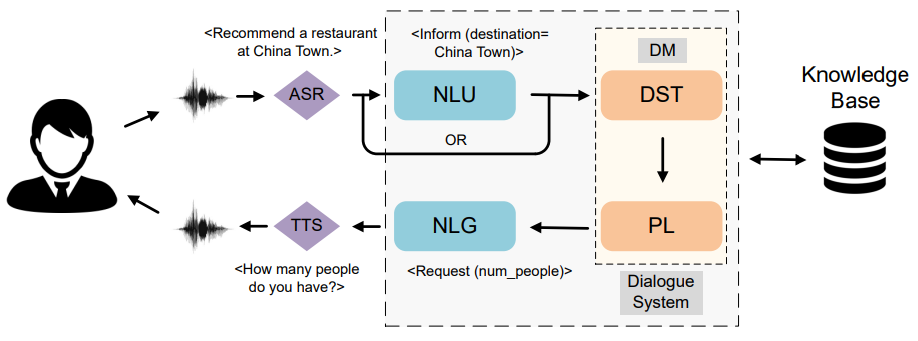
\includegraphics[scale=0.55]{Fig/pipeline_dialogue_system.png}
	\caption{\label{pipeline_dialogue_system}管道式对话系统结构示意图\cite{DBLP:journals/air/NiYPXC23}。}
\end{figure}

自然语言理解模块对原始的用户输入进行领域分类和意图识别,并提取其关键信息填入槽位中。
Deng等人\cite{DBLP:conf/slt/DengTHH12}和Tur等人\cite{DBLP:conf/icassp/TurDHH12}使用深凸网络将过去时间步的预测和当前消息结合起来,成功提高对话意图识别的准确率。
Sarikaya等人\cite{DBLP:journals/taslp/SarikayaHD14}使用受限玻尔兹曼机和深度置信网络初始化深度神经网络参数,解决了深度网络难以在领域分类和意图识别任务上训练的问题。
Ravuri等人\cite{DBLP:conf/interspeech/RavuriS15}利用循环神经网络(RNN)在序列预测上的优势,使用RNN对用户消息进行编码,以实现意图识别和领域分类。
Hashemi等人\cite{hashemi2016query}使用卷积神经网络(CNN)提取对话的多层级文本特征,以实现意图识别,同时该工作说明了CNN在序列预测任务上的可用性。
Lee等人\cite{DBLP:conf/naacl/LeeD16}使用RNN和CNN整合对话历史,获得上下文信息作为额外输入补充,解决了短语句信息不足的问题。
Wu等人\cite{DBLP:journals/corr/abs-2004-06871}提出预训练的面向任务对话BERT(TOD-BERT)模型提升意图识别任务上的准确率,同时所提出模型展现出小样本学习能力,缓解特定领域数据匮乏的问题。

对话状态跟踪模块根据当前用户消息和对话历史控制对话状态,以生成信息用于决定下一步动作。
Henderson等人\cite{DBLP:conf/sigdial/HendersonTY13}将深度学习模型用于对话状态跟踪,他们集成多种特征工程方法来预测每个槽-值对的概率。
Mrksic等人\cite{DBLP:conf/acl/MrksicSTGSVWY15}将RNN应用于对话状态跟踪以获得对话上下文感知。
随后,Mrksic等人\cite{DBLP:conf/acl/MrksicSWTY17}提出一种多跳的神经网络对话状态跟踪器,它使用系统输出、用户消息、候选槽值对作为输入,并基于对话历史对当前槽值对进行二分类预测。但是上述方法基于预定义的槽名与槽值,每一轮对话都需要对所有槽分别进行一次二分类,系统响应慢。
为了解决填槽类别多导致的计算复杂度高的问题,Lei等人\cite{DBLP:conf/acl/KanHLJRY18}提出信念片段,即一种与槽名相对应的对话上下文片段,通过构建一个两阶段CopyNet网络来拷贝和存储对话历史中的槽值,并用以生成回答,促进端到端训练,有效提升了系统在未登录词(OOV)下的准确度。
Wang等人\cite{DBLP:conf/emnlp/WangGZ20}提出了一种基于BERT模型的槽值预测方法,使用槽位注意力方法对相关片段进行检索,并使用槽值归一化方法将片段转化为最终的槽值。

对话策略学习模块根据对话状态决定下一步行为,主流方法是监督学习和强化学习。
Zhang等人\cite{DBLP:conf/acl/ZhangLGC19}提出一种高效资源调度方法,充分利用用户交互,在训练时使用概率调度器来分配对话样本,同时利用一个控制器决定使用真实样本还是模拟样本,有效提升强化学习训练的效果。
Takanobu等人\cite{DBLP:conf/acl/TakanobuLH20}提出一种多机对话策略学习方法,分别使用两个机器人扮演用户和系统,同时学习对话策略,同时,他们还加入特定角色的强化学习反馈,促进角色回答的生成。
Huang等人\cite{JSJX200408010}提出基于槽特征有限状态自动机的对话管理方法,通过树形的意图分层结构,实现多主题对话系统的主题检测与主题切换功能,并具有一定扩展性。

自然语言生成模块将系统的行为转化为自然语言,即最终输出,并返回给用户。
Wen等人\cite{DBLP:conf/sigdial/WenGKMSVY15}提出一种基于RNN的统计语言模型,通过语义约束和语法树学习回答生成,同时还使用CNN对候选回答进行排序,选出最佳回答。
Wen等人\cite{DBLP:conf/naacl/WenGMRSVY16}对循环语言模型采取先在大规模通用语料上预训练,然后在小规模特定领域语料上微调的训练方法,有效提升了循环语言模型的领域适应能力。
Li等人\cite{DBLP:conf/acl/LiYQCLL20}提出一种迭代矫正网络以迭代式修正所生成的标识符,首先使用监督学习训练网络,然后通过强化学习进行微调,并将槽位不一致的惩罚项添加到训练奖励中。

总结:管道式对话系统利用神经网络模型进行信息抽取和文本分类,而对话流程基于人工预定义的模板,因此特征相对固定,难以实现领域迁移。

\subsection{端到端式对话系统}

随着GPT\cite{DBLP:conf/nips/BrownMRSKDNSSAA20},BERT\cite{DBLP:conf/naacl/DevlinCLT19},T5\cite{DBLP:journals/jmlr/RaffelSRLNMZLL20}等序列到序列(Seq2Seq)\cite{DBLP:conf/nips/SutskeverVL14,DBLP:conf/emnlp/ChoMGBBSB14}预训练模型的兴起,基于Seq2Seq模型的端到端对话系统(End-to-End Dialogue System)逐渐成为主流。这类方法将对话系统的核心功能隐式地集成到一个复杂的神经网络模型当中,降低了系统模块复杂度。从研究侧重点上来看,端到端式对话系统的研究可分为两类:(1)基于模型架构的研究;(2)基于训练方法的研究。

Sordoni等人\cite{DBLP:conf/cikm/SordoniBVLSN15}提出一种上下文感知的Seq2Seq模型HRED,该模型同时学习字符级和对话级的文本表示,有效解决上下文感知的在线查询建议问题,提供少见且高质量的结果。
Serban等人\cite{DBLP:conf/aaai/SerbanSLCPCB17}进一步提出VHRED模型,对序列间的复杂依赖进行建模,通过在解码器中增加一个隐变量,在回答的多样性、长度和质量上都有一定的提升。
Weston等人\cite{DBLP:journals/corr/WestonCB14}提出一种记忆网络,使用RNN网络在每个时间步上向后传递历史信息。然而,这种模型包含五个模块,每个模块都需要单独进行监督训练,因此不适用于端到端式对话系统。
Sukhbaatar等人\cite{DBLP:conf/nips/SukhbaatarSWF15}在他们的工作基础上,提出了一种端到端的记忆网络,引入注意力方法,依次进行权重计算、记忆选择、最终预测。
在某些对话场景下,对话系统需要直接从用户输入中引用或摘要内容,而传统Seq2Seq模型的输出维度受限于输入的维度。
为解决该问题,Oriol等人\cite{DBLP:conf/nips/VinyalsFJ15}提出Pointer Net,每个时间步的输出都来自输入序列,将标识符预测问题转化为位置预测问题,以适应输入长度的变化。
然而,Pointer Net仅从输入中选择标识符的局限性较大,Gu等人\cite{DBLP:conf/acl/GuLLL16}提出CopyNet,在解码阶段的每个时间步中,决定复制输入中的标识符还是生成一个新的标识符,将复制概率和生成概率加和,得到最终的预测概率。
Balakrishnan等人\cite{DBLP:conf/acl/BalakrishnanRUW19}提出一种约束解码模块,以提升对话系统所生成回答的语义准确性。
Chen等人\cite{DBLP:conf/acl/ChenXX19}使用两个长期记忆模块分别存储知识元组和对话历史,然后用一个工作记忆模块来控制标识符的生成,有效提升对话相关知识的检索精确度。
Gao等人\cite{DBLP:conf/acl/GaoZOY20}使用一个释义模型对回答生成模型进行增强,释义模型与整个对话系统联合训练,用于增强训练样本。

Wang等人\cite{DBLP:conf/acl/WangZLHZL19}提出一种基于增量学习的训练方法,通过构建一个不确定性估计模块,在模型所生成回复的自信度低于阈值时使用人类回答作为结果,同时通过在线学习拟合人类回答,有效提升了模型回复质量。
Dai等人\cite{DBLP:conf/acl/DaiLTLSZ20}使用模型无关的元学习方法,仅依靠少量训练样本,在真实线上服务场景下有效提升模型的迁移能力和可靠性。
He等人\cite{DBLP:conf/emnlp/HeYYLSX20}提出一种“双教师单学生”知识蒸馏训练框架,首先两个教师模型分别以知识检索和回答生成作为训练目标,进行强化学习训练,然后让学生模型模仿教师模型的输出,实现专业知识的迁移。
Zhang等人\cite{DBLP:conf/acl/ZhangSGCBGGLD20}使用GPT-2\cite{radford2019language}作为基座模型,在Reddit社交媒体语料上训练,并引入最大互信息(MMI)评分函数,使对话系统能生成更相关、内容丰富、上下文一致的回复。
Daniel等人\cite{DBLP:journals/corr/abs-2001-09977}提出基于Evolved Transformer的Meena架构模型,将模型参数量扩充至2.6B,同时提出对话评估指标SSA,包含逻辑性和特异性两个维度,适用于对话模型的大规模人工评估场景,具有易于理解、一致性高等优势。
Roller等人\cite{DBLP:conf/eacl/RollerDGJWLXOSB21}使用具有特定对话能力的BST数据集对预训练模型进行微调,得到BlenderBot模型,BST数据集涵盖引人入胜、善于倾听、博学、同理心、有个性等对话能力,同时对比了检索式、生成式、混合式三种基于Transformer的模型架构,最终生成式模型的表现超过当时的最先进方法。
Bao等人\cite{DBLP:conf/acl/BaoHWWW20}提出对话行为隐变量,用以表征不同的说话风格,进而生成多样的回答,使用该方法在对话语料上训练BERT得到PLATO模型,该模型具备多轮流畅对话能力。

总结:端到端式对话系统的架构相对简单,且生成的回复更多样。然而,这类对话系统通常需要大量高质量对话语料,且模型尺寸一般比较大,训练资源开销大。

\section{面向垂直领域的对话生成}

垂直领域的对话内容相较于开放域对话具有更强的知识性与复杂性,直接使用开放域对话生成的方法无法得到准确可靠的回复。为此,许多研究者对面向垂直领域的对话生成展开研究。面向垂直领域的对话生成方法主要分为两类:(1)基于外部知识的方法;(2)基于知识注入的方法。

\subsection{基于外部知识的垂直领域对话生成}

Lin等人\cite{DBLP:conf/acl/LinJHWC20}提出基于拷贝机制的知识对话方法KIC,将循环知识交互解码器与知识感知的Pointer Net相结合,实现知识生成和知识拷贝。
Wu等人\cite{DBLP:conf/acl/WuLZZW20}采用一个多类别分类器对生成的单词、生成的知识实体和拷贝的查询单词进行融合,提升了模型生成回答的准确性、一致性和知识性。
Majumder等人\cite{DBLP:conf/emnlp/MajumderJBM20}同时进行角色信息选择和基于角色的响应生成,并使用强化学习训练对话智能体。
Moon等人\cite{DBLP:conf/acl/MoonSKS19}结合知识图谱与对话系统,将知识图谱信息作为外部知识,在强化学习框架中,智能体基于当前节点和状态选择相应的边,然后将知识组合到回答生成过程中。
Xu等人\cite{DBLP:conf/acl/XuWNWCL20}将知识图谱作为外部知识,控制粗粒度的对话生成,对话具有常识性知识支撑,使得智能体能更好地引导对话话题。
Jung等人\cite{DBLP:conf/emnlp/JungSL20}提出双向图探索模型AttnIO,用于在结构化知识图谱中检索外部知识,通过在遍历的每一步中计算注意力权重,使得模型能够选择更大范围的知识路径。
Yang等人\cite{DBLP:conf/emnlp/YangZE20}提出基于知识图谱的对话方法GraphDialog,首先将对话历史解析为依赖关系树,并编码为嵌入向量,然后使用注意力机制对知识图谱进行多跳推理,最后由解码器从图谱中拷贝实体或预测单词,实现将垂直领域知识图谱中的外部知识整合到模型回复中。
Lv等人\cite{SJSJ202312037}提出嵌入知识语义的医疗领域对话系统,使用BERT融合BiLSTM的对话训练方法,将医疗知识图谱的语义信息融入对话系统。

总结:基于外部知识的垂直领域对话生成方法主要基于符号逻辑或知识图谱来实现外部知识的补充。然而,这类方法无法有效建模未见过的实体,且没有考虑互联网上大量的文本信息,导致泛化性和实时性不足。

\subsection{基于知识注入的垂直领域对话生成}

Wu等人\cite{DBLP:journals/corr/abs-2303-17564}提出BloombergGPT金融大模型,使用通用语料与金融领域语料混合的数据集,从头训练领域大模型,在模型学习基本语言语法和世界常识的同时,注入垂直领域知识。然而,从头开始预训练大模型需要收集大规模的通用语料,同时提高模型后续在语言层面的迁移难度。因此,较为主流的知识注入方式是在预训练通用模型的基础上进行继续预训练或监督微调。
Zhang等人\cite{DBLP:conf/cikm/ZhangY23}提出XuanYuan金融领域大模型在预训练语言模型Bloom的基础上使用混合数据继续预训练,混合数据包含通用领域数据和金融领域内的专业知识数据,并采用Hybrid-Tuning训练策略,在提升模型领域内能力的基础上,保证模型通用能力不会退化。
Meng等人\cite{DBLP:conf/sigir/MengRCSRTR20}提出DukeNet,构建了一个双向知识交互网络,实现面向垂直领域知识的对话生成。
Chen等人\cite{DBLP:journals/corr/abs-2310-15896}提出扁鹊模型,通过构建高质量的医学领域对话数据集,得到预训练模型在下游对话任务上的良好性能。
Zhou等人\cite{DBLP:conf/acl/ZhouZHHZ20}提出KdConv,即中文多领域知识驱动对话数据集,通过在数据集上训练将知识注入模型中。
上述方法都需要构建大规模高质量领域内训练语料,对于垂直领域对话生成任务,往往还需要耗费人力,将其处理为“指令-回答”格式的对话数据,因此高质量的领域对话数据集十分稀缺。为解决数据稀缺的问题,Wang等人\cite{DBLP:conf/acl/WangKMLSKH23}提出Self-Instruct方法,利用大型语言模型对小规模的种子样本进行数据扩充,以生成更多符合要求的微调数据。
Zhang等人\cite{DBLP:journals/corr/abs-2305-11952}提出Self-QA方法,直接基于非结构化文档数据生成指令数据,无需初始种子数据,进一步降低了数据扩充的人力成本。
Wang等人\cite{DBLP:journals/corr/abs-2304-06975}提出Self-KG方法,基于中文医药知识图谱CMeKG生成指令数据,利用知识图谱中的节点关联信息,生成更高质量的指令数据。

总结:基于知识注入的垂直领域对话生成方法需要收集大规模高质量对话语料用于训练,同时知识被隐式存储在模型参数中,难以及时更新。

\section{基于大型语言模型的对话生成}

近年来,随着ChatGPT\cite{DBLP:conf/nips/Ouyang0JAWMZASR22}的发布,国内外先后出现许多预训练大型语言模型,如ChatGLM\cite{DBLP:conf/iclr/ZengLDWL0YXZXTM23}、文心一言\cite{DBLP:journals/corr/abs-2107-02137}、通义千问\cite{DBLP:journals/corr/abs-2309-16609}、LLaMA\cite{DBLP:journals/corr/abs-2302-13971}、百川\cite{DBLP:journals/corr/abs-2309-10305}等。因此,越来越多的研究者将大型语言模型作为对话生成研究的基础。
基于大型语言模型的对话生成可分为两类:(1)基于提示词工程的方法;(2)基于监督数据微调的方法。

\subsection{基于提示工程的对话生成}

Radford等人\cite{radford2019language}提出Zero-shot提示方法,利用大型语言模型进行范式迁移,无需训练即可让预训练模型完成下游任务,但该方法得到的输出可能不够准确或不符合预期。
为此,Brown等人\cite{DBLP:conf/nips/BrownMRSKDNSSAA20}提出Few-shot提示方法,在模型输入中提供高质量的示例,提升模型在复杂任务上的性能。
Wei等人\cite{DBLP:conf/nips/Wei0SBIXCLZ22}提出思维链(Chain-of-Thought,CoT)提示方法,通过在模型输入的结尾引导模型一步步思考,并在给出回复前先对问题进行拆解和分析,使得模型最终输出的答案更加准确。
Wang等人\cite{DBLP:conf/iclr/0002WSLCNCZ23}引入自洽性(Self-Consistency)解码策略,通过采样生成多条推理链,然后采用投票方法从这些推理链中选出一致性最高的答案,在GSM8K复杂推理数据集上,Self-Consistency相比于CoT方法有17.9\%的提升,证明该方法能很好的提升LLM的复杂任务推理能力。
Long等人\cite{DBLP:journals/corr/abs-2305-08291}提出思维树(Tree-of-Thought,ToT)提示方法,ToT是对CoT方法的扩展,通过管理树结构的中间推理步骤,同时使用深度优先或广度优先等搜索算法,对推理链路进行系统性扩展,使模型在得到错误答案时能够进行回溯,ToT在24类游戏任务上取得了74\%的成功率,而CoT仅有4\%。
Yao等人\cite{DBLP:journals/corr/abs-2305-16582}提出思维图(Graph-of-Thought,GoT)提示方法,使用基于图的架构,更好地适应人类非线性思考地特性。这类方法不需要重新训练模型即可提升模型性能,但提升受限于预训练模型自身的能力上限。

总结:提示工程方法的复杂度和成本相对较低,具有较高的灵活性,但生成的结果准确性受限于基座模型自身的能力,通常会出现不符合事实的回答,难以应对垂直领域对话。

\subsection{基于检索增强的对话生成}

大型语言模型具有良好的自然语言理解和自然语言生成能力,但往往面临幻觉问题,即回复内容不符合事实,甚至胡编乱造。这可能是因为模型在预训练阶段记忆了错误的知识,或是推理时的输入是预训练阶段没有遇到过的长尾知识。
针对后者,Lewis等人\cite{DBLP:conf/nips/LewisPPPKGKLYR020}提出检索增强生成(Retrieval Augmented Generation,RAG)技术,通过构建本地知识库,在对话阶段从知识库中召回与用户问题相关的文档,作为外部知识辅助语言模型给出回复,很好地缓解了大型语言模型的幻觉问题和实时性不足的问题。
Wang等人\cite{DBLP:conf/emnlp/WangYW23}提出Query2doc方法,利用大型语言模型对用户问题生成伪文档,以提升知识库的召回准确度,以减少无关文档对语言模型回复产生噪声干扰。
Jagerman等人\cite{DBLP:journals/corr/abs-2305-03653}在Query2doc方法的基础上提出思维链技术与伪相关反馈(Pseudo-Relevance Feedback,PRF)算法相结合的方法,在多个基准数据集上获得了超过Query2doc方法的效果。
Liu等人\cite{DBLP:journals/corr/abs-2307-03172}的研究表明,当相关信息出现在模型输入上下文的开头或结尾时,模型的性能最好,相关信息出现在中间位置时模型表现最差,且随着输入上下文的增长,模型性能显著下降,表明模型很难从长输入上下文中检索和使用相关信息。因此召回的知识文档数量及其在模型输入中的位置对模型性能至关重要。
Asai等人\cite{DBLP:journals/corr/abs-2310-11511}提出Self-RAG方法,生成模型通过检索召回多个相关文档,并通过并行处理和排序选择最合适的回复。
Cui等人\cite{DBLP:journals/corr/abs-2306-16092}提出ChatLaw中文法律大模型,在RAG的基础上。融入法律意图识别、法律关键词提取等模块,满足法律相关领域的应用需求。这类方法在背景知识丰富且逻辑相对复杂的专业领域上表现不佳。

总结:检索增强方法能很好地改善大型语言模型的幻觉问题,得到高准确性的回复。然而,现有的检索增强方法更多的关注如何提升外部知识的召回准确性,没有考虑基座模型内部知识与外部知识之间的偏差,存在性能瓶颈。

\subsection{基于模型微调的对话生成}

根据研究目标的不同,基于模型微调的方法主要可分为两类:(1)参数高效的微调方法;(2)人类偏好对齐的微调方法。

Houlsby等人\cite{DBLP:conf/icml/HoulsbyGJMLGAG19}提出适配器微调(Adapter-Tuning)方法,在Tranformer层中插入小规模的神经网络模块,并在训练过程中冻结模型原有参数,仅更新这些适配器模块,实现与全量微调相近的性能。
Mahabadi等人\cite{DBLP:conf/nips/MahabadiHR21}提出Compacter方法,通过结合超复数乘法和参数共享,将模型原有的线性层视为两个小矩阵的Kronecker积,实现在不损害模型性能的情况下显著减少适配器参数量。
Pfeiffer等人\cite{DBLP:conf/eacl/PfeifferKRCG21}提出AdapterFusion方法,先分别训练任务特定的适配器,再将不同任务的适配器融合起来,以利用跨任务知识来提升迁移学习的性能。
除了在Transformer模型内部引入额外的神经网络模块外,也有研究人员在模型输入中引入额外的可训练上下文,实现参数高效微调。
Li等人\cite{DBLP:conf/acl/LiL20}提出Prefix-Tuning方法,在模型输入首端增加一个连续的、任务相关的嵌入向量来进行训练,在显著减少训练参数量的情况下提升模型在自然语言生成任务上的性能。
% 与Prefix-Tuning思想相似,Brian等人\cite{lester-etal-2021-power}提出提示学习(Prompt Tuning)方法,通过在输入中插入一段任务特定的、可被训练的离散提示词元,获得了与微调相近的效果,同时超过了人工设计提示词的性能。
Liu等人\cite{DBLP:journals/corr/abs-2110-07602}在Prefix-Tuning的基础上,进一步提出P-Tuning v2方法,在模型的每一层上都加上了可训练的层级提示词元,且对于不同难度的任务使用不同的提示长度。
Gu等人\cite{DBLP:conf/acl/GuHLH22}提出PPT方法,在模型与训练阶段插入软提示,以寻找更合适的参数初始化起点。
Lee等人\cite{DBLP:journals/corr/abs-1911-03090}仅微调BERT和RoBERTa模型最后四分之一的中间层,冻结模型其他参数,达到了全量微调方法90\%的性能。
Zaken等人\cite{DBLP:conf/acl/ZakenGR22}提出BitFit方法,仅对模型中的bias参数进行优化更新,并通过实验证明该方法在多个评测集上能够达到超过95\%的性能。
除了通过人工指定的方式确定需要更新的模型参数子集外,Zhao等人\cite{DBLP:conf/emnlp/ZhaoLMJS20}提出基于二维矩阵的掩码方法,通过学习掩码,自动选择需要更新的关键参数。
Aghajanyan等人\cite{DBLP:conf/acl/AghajanyanGZ20}通过实验发现,模型全参数微调的过程可以被重新参数化为一个低维子空间的优化过程。
Li等人\cite{DBLP:conf/iclr/LiFLY18}提出内在维度(intrinsic dimension)概念,用于衡量使模型达到预期性能所需要更新的最小参数量,并通过实验证明较低的内在维度重新参数化即可达到全量微调超过85\%的性能,同时发现内在维度随模型尺寸增大而减小,且模型预训练过程能够隐式减小其内在维度。
Hu等人\cite{DBLP:conf/iclr/HuSWALWWC22}提出了低秩自适应(Low-Rank Adaptation,LoRA)方法,通过使用低维结构来近似大模型的高维结构,以降低模型训练的复杂度和计算开销。
Qiu等人\cite{DBLP:journals/corr/abs-2110-07867}进一步提出假设,认为多任务自适应存在一个通用的内在空间,因此能够将多任务学习过程重新参数化为一个低维内在子空间的优化过程。
总体来说,基于监督数据微调的方法性能优于基于提示词工程的方法,但存在高质量标注数据难获取的问题。

Long等人\cite{DBLP:conf/nips/Ouyang0JAWMZASR22}提出基于人类反馈的强化学习(Reinforcement Learning with Human Feedback,RLHF)算法,其工作过程包括采集高质量数据集对语言模型监督微调(SFT)、收集人类偏好排名数据集并训练奖励模型(RM)、执行近端策略优化(Proximal Policy Optimization,PPO)强化学习。
该算法能够很好地帮助模型生成符合人类偏好的回复,同时减少生成式模型中的偏见。然而,RLHF算法在PPO强化学习训练阶段需要同时使用四个大型语言模型,导致训练计算资源开销大,同时PPO强化学习过程不稳定,导致模型难以训练。为此,许多研究者提出其他的人类偏好对齐算法替代RLHF算法。
Li等人\cite{DBLP:journals/corr/abs-2309-07124}提出RAIN可回滚自回归推理算法,利用语言模型评估自己生成的结果,并用评估结果来指导语言模型输出,以确保输出符合人类偏好,无需微调即可实现语言模型与人类偏好的对齐。
Zheng等人\cite{DBLP:journals/corr/abs-2307-04964}针对PPO训练不稳定的问题,通过实验探索了PPO训练中最关键的技巧,并用PPO-max表示这套最佳实现方式。
Dong等人\cite{DBLP:journals/corr/abs-2304-06767}提出RAFT方法,在采集的人类偏好数据中选取多个高质量样本,继续对SFT模型进行监督微调,利用更多次采样和更少的梯度计算,让模型更稳定和鲁棒。
Yuan等人\cite{DBLP:journals/corr/abs-2304-05302}在RLHF的基础上提出RRHF算法,直接使用偏好数据训练语言模型,结合排名损失和SFT损失,在性能上与PPO方法相近,但实现相对简单且训练稳定。
Cheng等人\cite{DBLP:journals/corr/abs-2311-04155}提出BPO黑盒提示优化算法,通过采集人类偏好数据,训练提示优化器,对用户指令进行优化,使模型生成的内容更符合用户期望。
Rafailov等人\cite{DBLP:conf/nips/RafailovSMMEF23}提出DPO算法,其思想与RRHF相似,但同时引入SFT模型的约束,保证在不使用SFT损失的情况下训练依然稳定,该方法在多个开源RM数据集上获得优于RLHF的奖励得分,且对超参数的敏感度更低,效果更稳定。
Liu等人\cite{DBLP:journals/corr/abs-2309-06657}提出RSO算法,使用拒绝采样得到高质量回答的分布。
上述方法依赖于人类反馈数据,标注成本高昂。为解决该问题,Bai等人\cite{DBLP:journals/corr/abs-2212-08073}提出RLAIF方法,用宪法人工智能(CAI)代替人类进行偏好的标记工作,实验表明RLAIF能够达到与RLHF相当的性能。
此外,Li等人\cite{DBLP:journals/corr/abs-2310-10505}提出ReMax算法,通过削减PPO中冗余庞大的计算开销,节省RLHF算法50\%的内存消耗,并加快2倍训练速度。现有方法一方面需要高昂的人力成本完成偏好数据标注,另一方面存在训练计算资源开销大、难训练的问题。
Wei等人\cite{DBLP:conf/iclr/WeiBZGYLDDL22}提出指令微调(Instruction Tuning)方法,通过监督训练,让语言模型学会按照指令要求完成任务,从而具备遵循指令的能力,即使面对训练中未曾见过的任务,模型也能够生成合适的回复。

总结:模型微调方法通过调整模型内部参数,能够控制模型内在的行为模式,对齐人类偏好,但是对动态数据缺乏实时性,难以及时跟进垂直领域的新知识。

\section{本章小结}

本章主要对研究相关的对话系统、面向垂直领域的对话生成以及基于大型语言模型的对话生成进行了介绍。总体而言,本章先介绍了对话系统在管道式对话系统和端到端式对话系统等方向的相关进展。然后,本章介绍了基于外部知识和基于知识注入的垂直领域对话生成方法的研究进展。最后,本章对基于大型语言模型的对话生成任务在基于提示工程、基于检索增强和基于模型微调方法的研究现状作了相关概述。 % 第二章
\chapter{基于内外部知识对齐的检索增强对话生成}

\section{问题描述}

基于大型语言模型的对话生成存在事实性、实时性不足的问题。现有方法主要通过检索增强生成方法进行垂直领域对话生成,以输入的形式将垂直领域知识引入对话模型中。然而,面对垂直领域中较难的问题时,模型往往不能很好理解知识文档中的复杂信息,导致检索增强效果不佳。语言模型在预训练中没见过垂直领域的长尾知识,因此检索增强所补充的知识文档可能未能与模型内部知识完全对齐。为此,本章研究如何对齐外部知识文档的垂直领域长尾知识和模型内部知识,进而使模型兼具事实性与垂直领域推理能力。同时,以金融分析领域为应用场景对算法进行验证。金融分析领域主要涵盖两个关键任务:(1)股票趋势预测任务;(2)金融问答任务。

对于股票趋势预测任务,给定一组公司$C=\{c_i\}_{i=1}^N$以及对应的知识文档$D=\{d_j\}_{j=1}^M$,对话系统给出该股票的未来趋势预测:
\begin{equation}
	Pred_i=\pi(c_i, d_j), Pred_i \in \{up, down\}
\end{equation}
其中,$\pi$表示股票预测系统,$d_j$是检索得到的与公司$c_i$相关的知识文档。目标是选择出一批被预测股价会上涨的公司:
\begin{equation}
	C_{chosen} = \{c_i | c_i \in C \land Pred_i = up\}
\end{equation}
目前机器学习和深度学习的方法已经被广泛应用在该任务上,并取得了一定的进展。然而,这些方法通常只能基于过去的市场价格数据预测未来股票的涨跌,而无法给出具体的分析过程和原因,其预测结果对投资者用户来说缺乏可解释性。同时,这类方法难以将新闻、研报等非结构化的文本信息用于股票趋势预测中。

对于金融问答任务,我们将一个多轮对话视为两个对话者之间的诸多“问题-回复”对。令$Q_t$和$R_t$表示在第$t$轮对话时的用户问题和系统回复,$H_t=[Q_0, R_0, …, Q_{t-1}, R_{t-1}]$作为对话历史。我们将金融问答任务的形式定义为,给定对话历史、用户问题和检索到的相关文档,对话系统$\pi$能够给出相应的回复:
\begin{equation}
	R_t = \pi(d_k, H_t, Q_t)
\end{equation}
其中,$d_k$表示检索到的与$Q_t$相关的知识文档。
目前大部分的金融问答方法主要基于大型语言模型,这类模型在大规模语料上经过预训练,具有强大的文本理解和文本生成能力。但由于金融领域数据集的稀缺性和模型微调的知识滞后性,语言模型存在不可控的“幻觉”问题,即编造没有现实基础的事实或细节。因此,一些基于检索增强生成的方法提出利用知识库检索出与用户查询相关的外部知识辅助模型生成回答,一定程度上缓解了大型语言模型的幻觉问题和实时性问题。然而,对于某些金融领域问题,涉及到广泛的金融背景知识,仅依靠知识库检索得到的知识文档并不足以让模型给出正确的分析和解答。

\section{基于内外部知识对齐的检索增强对话生成}
\subsection{算法总体框架}

针对以上问题,本章提出基于内外部知识对齐的检索增强对话生成方法。整体算法框架如图\ref{rag_framework}所示,整个框架主要包括三个部分:(1)对金融知识文档进行多粒度语义切分,得到一系列金融知识文档块,并构建外部知识库用于存储和检索这些知识文档块;(2)构建AlphaFin金融数据集,为模型注入金融领域的内部知识,同时与知识库中的外部知识进行对齐;(3)利用多级混合检索,对用户查询和知识库中的文档块计算语义相似度,得到与用户查询相关性最高的一系列文档块,最后与指令提示词拼接输入模型,得到回答。

\begin{figure}[htbp]
	\centering
	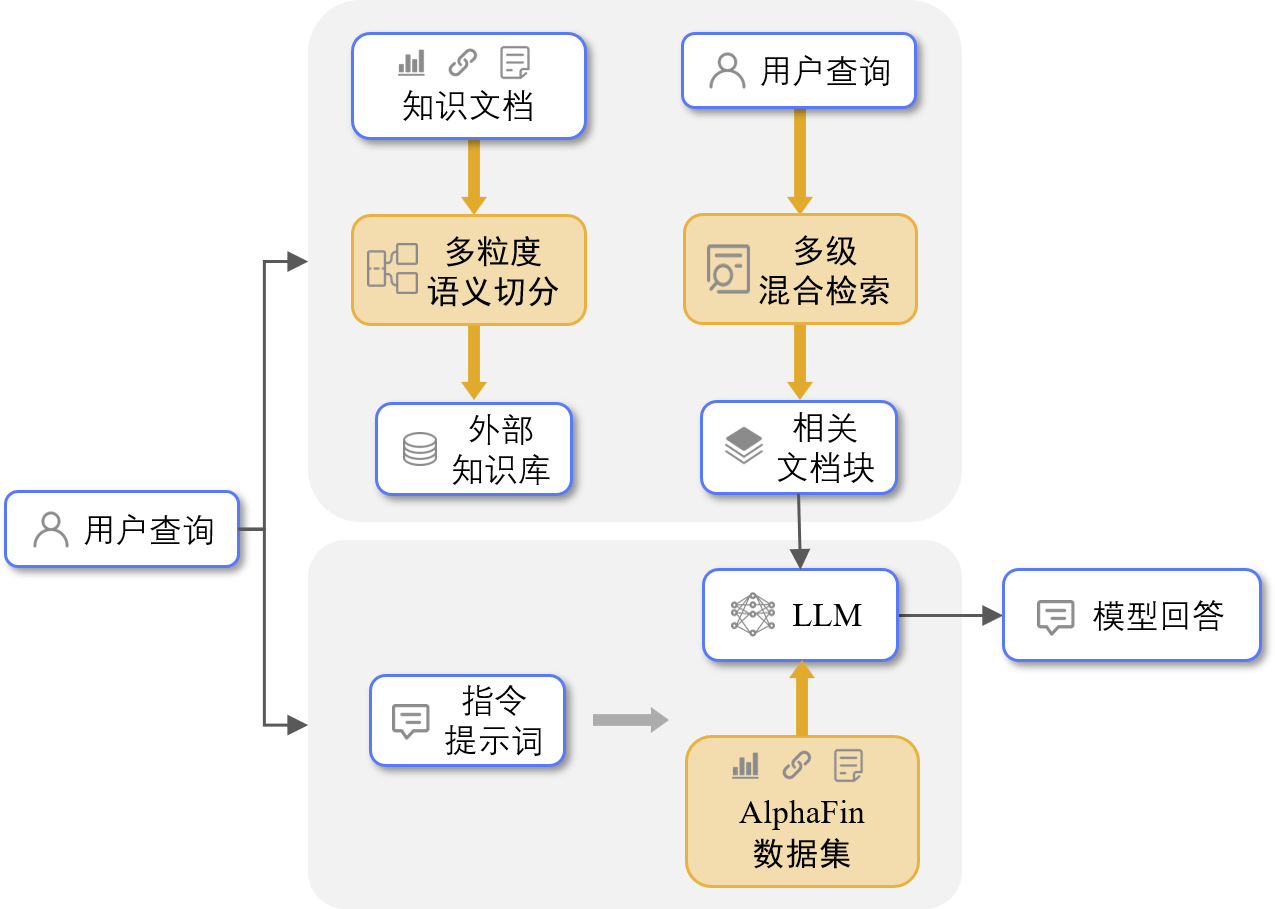
\includegraphics[scale=0.7]{Fig/rag_framework.png}
	\caption{\label{rag_framework}本章所提出的检索增强对话生成框架示意图。}
\end{figure}

\subsection{多粒度语义切分模块}

如图\ref{split_chunk_module}所示,外部知识库的构建是检索增强生成中的的重要组成部分,用于高效存储和检索相关知识文档。

\begin{figure}[htbp]
	\centering
	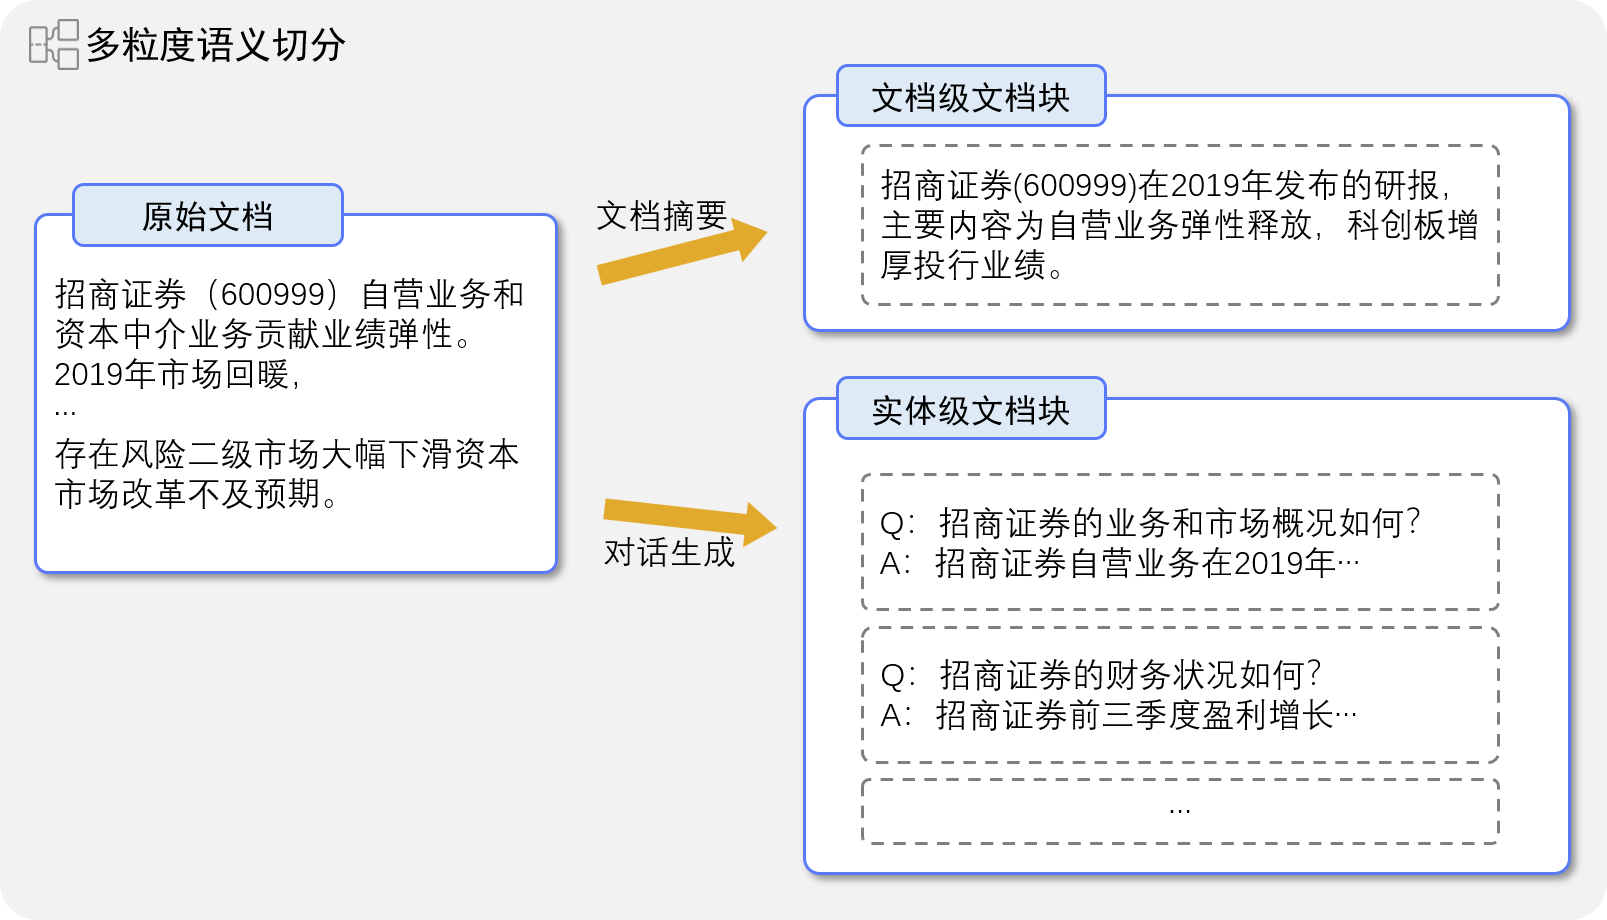
\includegraphics[scale=0.5]{Fig/split_chunk_module.png}
	\caption{\label{split_chunk_module}对话框架中的多粒度语义切分模块示意图。}
\end{figure}

为了提升知识库召回文档的准确度和效率,本章节对原始知识文档进行多粒度语义切分,从文档中提取出关键信息。如图\ref{split_chunk_module}所示,我们采用两种切分策略:粗粒度文档级总结和细粒度实体级对话生成。其中,语义切分过程使用大型语言模型(如ChatGPT模型)通过设计相应的提示词完成,本文所使用的提示词如表\ref{gen_finqa_prompt}所示。

\begin{table}
	\caption{\label{gen_finqa_prompt}实体级对话生成所使用的提示词。}
	\centering{}%
	\small 
	\begin{tabular}{c}
		\toprule[2pt]
		提示词\tabularnewline
		\hline 
		\begin{tabular}{l}
			基于<content>,请提出一个金融问题。 \\ 输入:<sequential data> \\ 输出:<question>
		\end{tabular} \\
		\bottomrule[2pt]
	\end{tabular}
\end{table}

对于文档$d_k$,其语义切分过程如下:
\begin{equation}
	s_k = LLM_{sum}(d_k)
\end{equation}
\begin{equation}
	(q_{k0}, a_{k0}), (q_{k1}, a_{k1}), \dots = LLM_{qa}(d_k)
\end{equation}
其中,$s_k$表示文档$d_k$的摘要,$(q_{k\_}, a_{k\_})$是所生成对话的“问题-回答”二元组。例如,假设$d_k$是与“股票k线”相关的文档,$q_{k\_}$则可能是“股票k线是什么?”。

我们以文档级摘要切分策略为例,给定文档摘要$s_k$,我们通过句子嵌入模型得到其嵌入向量$e_sk$。该向量将被存储在知识库中,作为数据库索引被用于后续的检索步骤。
\begin{equation}
	e_{sk} = SentEmbed(s_k)
\end{equation}
其中,$SentEmbed$是句子嵌入模型,如BGE、SGPT等。

\subsection{AlphaFin数据集构建}

\begin{figure}[htbp]
	\centering
	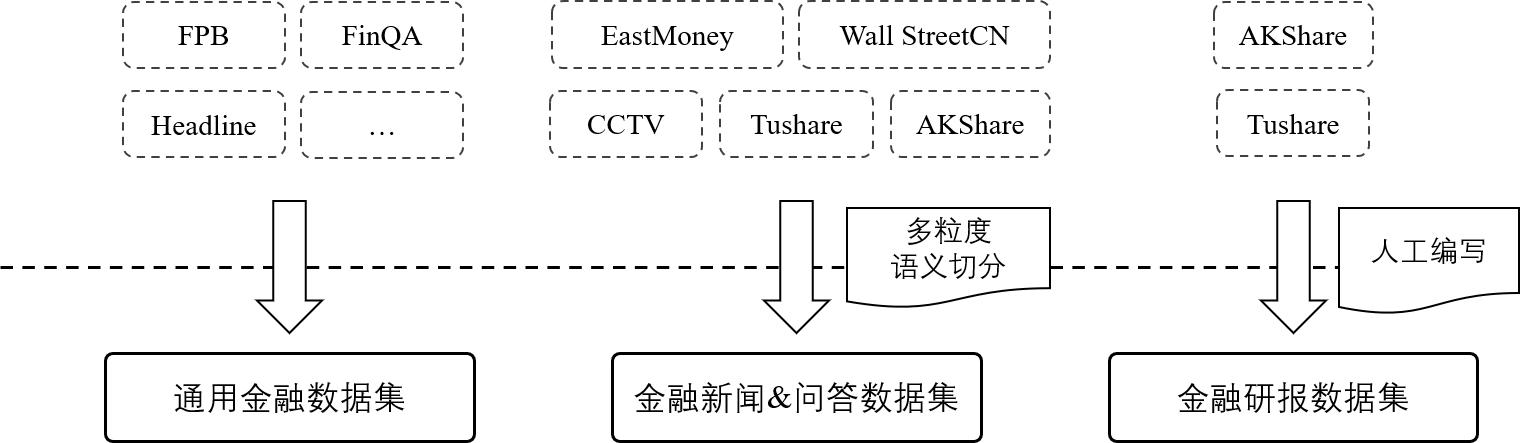
\includegraphics[scale=0.6]{Fig/dataset_process.png}
	\caption{\label{dataset_process}数据集预处理过程示意图。}
\end{figure}

如图\ref{dataset_process}所示,我们基于金融领域知识文档构建AlphaFin数据集,该数据集包含三部分:通用金融数据集、金融新闻与问答数据集、金融研报数据集。各数据集具体来源和预处理方式如下:

通用金融数据集:由传统金融开源数据集构成,如FPB\cite{DBLP:journals/jasis/MaloSKWT14}、FinQA\cite{DBLP:conf/acl/ZhuLHWZLFC20}、ConvFinQA\cite{DBLP:journals/corr/abs-2310-00566}、Headline\cite{DBLP:journals/corr/abs-2009-04202}等。这些开源数据集主要是英文数据集,因此我们从中采样一部分,用于增强模型的多语言能力、信息抽取能力和摘要能力。

金融新闻数据集:为模型提供真实世界的金融知识,我们整合了在线新闻资源,如CCTV的金融板块和华尔街见闻。利用ChatGPT\cite{DBLP:conf/nips/Ouyang0JAWMZASR22}提取每条新闻的摘要,构建金融新闻数据集。这个过程提高了模型为金融新闻生成汇总的能力。

金融问答数据集:这部分包含了Tushare\cite{tushare}和AKshare\cite{akshare}的股票价格和其他财务数据。它利用序列数据,例如真实世界的股票价格趋势(例如{…, 170, 173, 171, 175, 173, 170,…})。给定源数据以顺序格式呈现,我们利用ChatGPT和以下提示,在其上生成财务问题。

金融研报数据集:我们通过DataYes数据平台API构建了财务报告数据集,包括机构对公司进行的专业分析和知识。我们手动对齐公司的财务报告及其在报告发布当天的股票价格,并使用如表\ref{financial_report_format}格式来生成最终数据。其中,金融研报数据集包含两种类型的数据:1)Raw类型,样本输出中仅包含股票涨跌结果和涨跌概率;2)CoT类型,在给出股票涨跌预测结果前,先对输入中的公司研报和市场数据信息进行基本面和技术面的详细分析和逻辑推导,这部分CoT分析由金融领域专家人工编写,以保证其正确性和质量。

\begin{table}
	\caption{\label{financial_report_format}金融研报数据集样本格式。}
	\centering
	\begin{tabular}{c|c|c}
		\toprule[2pt]
		数据集 & Raw & CoT \\
		\hline
		系统指令 & \multicolumn{2}{l}{
			\begin{tabular}{p{12cm}}
				请根据下方提供的该股票相关研报与数据,对该股票的下个月的涨跌,进行预测,请给出明确的答案,“涨” 或者 “跌“。同时给出这个股票下月的涨跌概率,分别是:极大,较大,中上,一般。\\
			\end{tabular}
		} \\
		\hline
		输入 & \multicolumn{2}{l}{
			\begin{tabular}{p{12cm}}
				<|公司研报|> \\ 发布日期:<date> \\ 研报题目:<title> \\ 目标价格:<target price> \\ 研报摘要:<abstract> \\  \\ <|市场数据|> \\ 1.股票价格(元):<price>; \\ 2.日涨跌幅(\%):<change>; \\ 3.日成交量(亿):<volumn> \\
			\end{tabular}
		} \\
		\hline
		输出 & 
		\begin{tabular}{p{3.8cm}}
			这个股票的下月最终收益结果是:'跌',下跌概率:中上 \\
		\end{tabular} & 
		\begin{tabular}{p{8.2cm}}
			通过研报和市场走势数据可以得出以下结论: \\ 1、基本面: <basic analysis>。 \\ 2、技术面: <tech analysis>。 \\ 因此,我们预测,这个股票的下月最终收益结果是:'跌',下跌概率:极大 \\
		\end{tabular} \\
		\bottomrule[2pt]
	\end{tabular}
\end{table}

最终得到的AlphaFin数据集各组成部分的统计信息如表\ref{alphafin_info}所示,任务类型涵盖NLP基础任务、金融新闻、金融问答、研报分析,不同任务类型、不同语言的数据量相当,以保证模型学习到的各项能力趋于平衡。

\begin{table}
	\caption{\label{alphafin_info}AlphaFin数据集统计信息。}
	\centering
	\begin{tabular}{lccccc}
		\toprule[2pt]
		数据集 & 类别 & 大小 & 输入长度 & 输出长度 & 语言 \\
		\hline
		\multicolumn{2}{l}{通用金融数据集} & 42,373 & 712.8 & 5.6 & 英文 \\
		\hline
		\multirow{2}*{金融新闻\&问答数据集} & 新闻 & 21,000 & 1313.6 & 40.8 & 中文 \\
		~ & 问答 & 79,000 & 497.8 & 64.2 & 中文 \\
		\hline
		\multirow{2}*{金融研报数据集} & Raw & 120,000 & 2203.0 & 17.2 & 中文 \\
		~ & CoT & 200 & 2184.8 & 407.8 & 中文 \\
		\bottomrule[2pt]
	\end{tabular}
\end{table}

为了实现外部知识与模型内部知识的对齐,我们对LLM进行微调。首先,我们使用专业领域的知识文档构建两类数据集:通用QA数据集和CoT分析数据集。通用QA数据集的构建过程与3.2.2节中的细粒度实体级对话生成过程相同,其作用是让模型具备基本的专业领域理解能力;CoT分析数据集的构建需要先采集针对知识文档的专业领域问题,然后人工撰写CoT详细分析的专业解答,其作用是让模型具备专业领域的详细分析能力和文本生成能力。

LLM微调过程分为两个阶段:1)首先在通用QA数据集上进行微调,将专业领域的基本知识注入模型内部;2)然后在CoT分析数据集上进行微调,进一步对齐知识文档中的长尾知识与模型内部的知识。所有的微调过程均采用LoRA方法,以缓解训练过拟合问题,同时降低训练成本。微调后的LLM将作为对话框架中的对话生成模型,与用户交互。

\subsection{多级混合检索模块}

知识检索过程如图\ref{search_module}所示。从知识库中检索相关知识文档,首先将用户问题$Q$输入与3.2.2节相同的句子嵌入模型中,获得其嵌入向量$e_Q$。
\begin{equation}
	e_Q = SentEmbed(Q)
\end{equation}

依次计算用户文档嵌入向量$e_Q$与各文档嵌入向量$e_sk$的余弦相似度,选择相似度最高的文档作为外部知识,辅助LLM生成回复。
\begin{equation}
	d^* = \mathop{\arg\max}_{d_k}\frac{e_Q^\top \cdot e_{sk}}{|e_Q||e_{sk}|}
\end{equation}
其中,对于细粒度实体级对话生成的切分策略,上式中的$s_k$和$d_k$可分别被替换为$q_{k\_}$和$a_{k\_}$。

% TODO:补充BM25、RRF和Rerank

\begin{figure}[htbp]
	\centering
	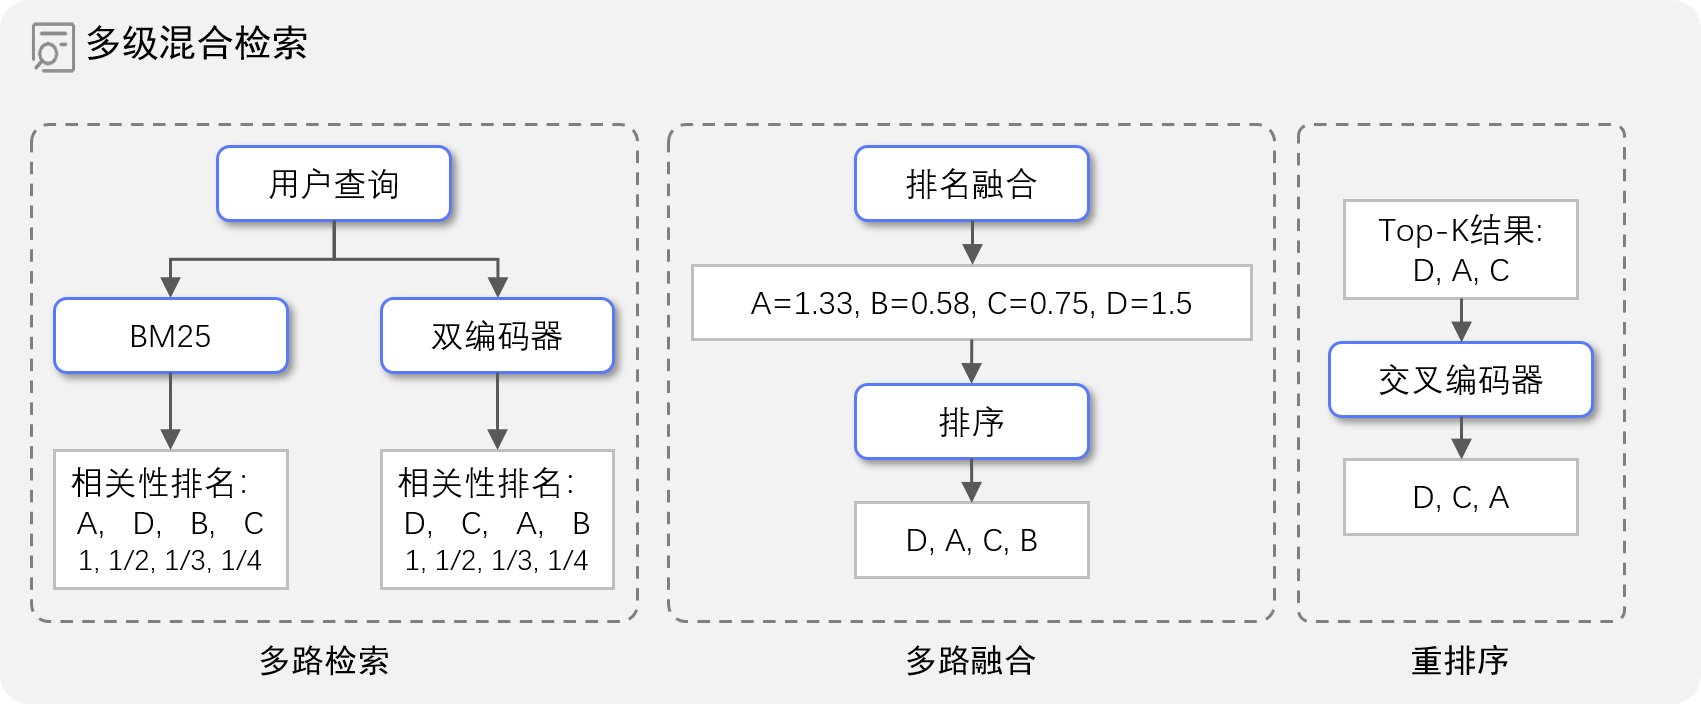
\includegraphics[scale=0.55]{Fig/search_module.png}
	\caption{\label{search_module}对话框架中的多级混合检索模块示意图。}
\end{figure}

\subsection{回答生成与后处理}

给定对话历史$H_t$,用户问题$Q_t$,以及检索到的与用户问题$Q_t$相关的文档$d^*$,目标是获得第$t$轮对话的回复$R_t$。然后,我们拼接提示词模板、知识文档、对话历史和用户问题,以得到LLM的输入$I_t$。将$I_t$传入LLM,即可得到回复$R_t$。
\begin{equation}
	I_t = concat(Prompt, d^*, H_t, Q_t)
\end{equation}
\begin{equation}
	R_t = LLM(I_t)
\end{equation}

如图所示,给定输入$I_i$,我们利用LLM来预测股票的涨跌趋势,这可以看作是一个二分类任务。通过将$I_i$输入LLM,得到关于$c_i$的回复文本$Res_i$。
\begin{equation}
	Res_i = LLM(I_i)
\end{equation}

然后,我们使用基于规则的方法从$Res_i$中提取出趋势预测结果$Pred_i$。最后,我们选择所有被预测为“上涨”的股票,得到股票集合$C_chosen$。
\begin{equation}
    Pred_i = \left\{ 
        \begin{array}{ll}
            up, & if\ \ ``up" \in Res_i \\
            down, & else \\
        \end{array}
    \right.
\end{equation}
\begin{equation}
	C_{chosen}={c_i | Pred_i = up}
\end{equation}

另外,我们按月滚动执行该投资策略。每个月,对于$C_chosen$中的所有股票$c_i$,我们会持有一整个月。投资组合中的每种股票的比例是通过市值加权计算得到的。
\begin{equation}
	AR_m = AR_{m-1} + \sum_{c_i \in C_{chosen}}\omega_{c_i} R_{c_i}
\end{equation}
其中,$AR_m$表示第$m$个月的累计收益,$R_{c_i}$表示股票$c_i$的收益。$\omega_{c_i}$代表股票$c_i$在投资组合中所占的比例。$v_i$是公司$c_i$的市值。
\begin{equation}
	\omega_{c_i} = \frac{v_i}{\sum_{c_n \in C_{chosen}}v_n}
\end{equation}

\section{实验}

在本节中,我们以金融领域为应用场景对算法进行实验验证。金融领域分析任务主要包括两个部分:1)股票趋势预测;2)金融问答。对于第一类任务,我们主要考察模型的对股票相关信息的理解能力和趋势预测能力,通过年化收益率和预测准确率体现。对于第二类任务,我们主要考察模型对用户问题解答的准确性、相关性、和有帮助性,通过人工偏好评价和GPT-4偏好评价体现。

\subsection{数据集介绍}

我们从数据源中选择训练集之外的一个数据子集作为测试集。鉴于所有的研究数据集都是英文的,我们的主要重点是从其他数据集采样。例如财务报告和StockQA数据集。对于阶段1,我们从财务报告数据集中选择测试数据集。一个例子演示如下:请判断公司的发展趋势,并给出一个明确的答案是上升还是下降。输入:<报表和股价>,输出:<上升/下降>。对于阶段2,测试数据集从StockQA和research数据集中采样。AlphaFin- test数据集使我们能够评估模型在资本市场上的能力。

\subsection{基准方法}

股票指数:我们选取了中国股票市场的指数,包括上证50(SSE50)上证指数(SCI)、沪深300(CSI300)和创业板指数(CNX)。

随机森林:随机森林是一种监督式学习算法,主要用于分类和回归问题,它是由多个决策树组成的集成模型。其核心思路是,当训练数据被输入模型时,并不是用整个训练数据集建立一个大的决策树,而是采用不同的子集和特征属性建立多个小的决策树,然后将它们合并成一个更强大的模型。

RNN:循环神经网络(Recurrent Neural Network,简称RNN)是一种特殊的神经网络,它能够处理序列数据,并利用序列中的历史信息进行学习。RNN的结构包含一个循环单元,这个单元允许信息在时间步骤之间传递,从而使得网络能够记忆和处理之前时刻的信息。

BERT:BERT是一种语言表示模型,BERT代表来自Transformer的双向编码器表示(Bidirectional Encoder Representations from Transformers)。BERT旨在通过联合调节所有层中的双向上下文来预训练深度双向表示。因此适用于文本理解、机器翻译等任务。

GRU:GRU(Gated Recurrent Unit)是一种门控循环单元,属于循环神经网络(RNN)的一种。它的主要特点是具有两个门:更新门(update gate)和重置门(reset gate)。更新门负责控制上一时刻状态信息对当前时刻状态的影响,而重置门负责控制忽略前一时刻的状态信息的程度。GRU是一种简单而有效的RNN变体,它在保持与LSTM相当性能的同时,减少了参数数量,提高了训练效率,因此在实际应用中常常被优先选择。

LSTM:LSTM(Long Short-Term Memory)是一种特殊的循环神经网络(RNN),它能够有效地捕捉和记忆长序列中的信息,克服了传统RNN中梯度消失或爆炸的问题。LSTM的核心结构包括四个部分:遗忘门、输入门、细胞状态和输出门。它通过门控机制控制信息的流动,从而在序列学习中表现出强大的能力。

逻辑回归:逻辑回归是一种统计学习方法主要用于二分类问题,即输出只有两种,分别代表两个类别。逻辑回归的优点包括速度快,适合二分类问题,简单易于理解,直接看到各个特征的权重,能容易地更新模型吸收新的数据。

XGBoost:XGBoost是一个优化的分布式梯度增强库,旨在实现高效,灵活和便携。它在 Gradient Boosting 框架下实现机器学习算法。XGBoost提供并行树提升(也称为GBDT,GBM),可以快速准确地解决许多数据科学问题。

决策树:决策树是一种树形结构,用于分类和回归问题,它通过一系列的判断(节点)和决策(边)来预测实例的类别。决策树的特点包括计算复杂度不高、输出结果易于理解、对中间值的缺失不敏感,可以处理不相关特征数据。此外,决策树是一种非参数的有监督学习方法,它能够从一系列有特征有标签的数据中总结出决策规则并用树状图的结构来呈现这些规则。

ChatGLM2-6B:ChatGLM2-6B是智谱AI及清华KEG实验室发布的中英双语对话模型。它使用了 GLM 的混合目标函数,经过了 1.4T 中英标识符的预训练与人类偏好对齐训练,在CEval、GSM8K等数据集上得到大幅度的性能提升。同时,ChatGLM2-6B使用了 Multi-Query Attention,提高了生成速度,同时也降低了生成过程中 KV Cache 的显存占用。同时,ChatGLM2-6B 采用 Causal Mask 进行对话训练,连续对话时可复用前面轮次的 KV Cache,进一步优化了显存占用。

ChatGPT:ChatGPT全名Chat Generative Pre-trained Transformer,是由OpenAI开发的一款基于人工智能技术的聊天机器人程序,于2022年11月30日发布。它基于GPT(Generative Pre-trained Transformer)架构,这是一种自然语言处理(NLP)模型,能够理解和生成人类的自然语言。

FinMA:FinMA是一个综合性金融大型语言模型(LLM)。它旨在理解复杂的金融语言和概念,并经过微调以遵循自然语言指令,提高其在下游金融任务中的性能。它使用自建金融数据集的完整指令数据进行训练,涵盖了NLP和预测任务。这使它成为一种更全面的模式,能够处理更广泛的金融任务。

FinGPT:FinGPT 是2023年6月哥伦比亚大学联合上海纽约大学推出全新大模型产品,这是一款面向金融领域的大模型产品。它使用自建金融数据集在llama2-13b、ChatGLM2-6B等预训练模型上进行LoRA微调,得到金融领域语言模型。本实验所使用的是基于ChatGLM2-6B的版本。

通义金融:通义金融-14B(Tongyi-Finance-14B)是针对对金融行业推出的大语言模型,基于通义千问基础模型进行行业语料增量学习,强化金融领域知识和场景应用能力,覆盖金融知识问答、文本分类、信息抽取、文本创作、阅读理解、逻辑推理、多模态、Coding等能力象限。

\subsection{评价指标}

对于阶段1,我们使用两类指标。第一类是核心指标,包括衡量盈利能力的ARR和ACC。第二类是辅助分析不同模型的辅助指标,如maximum drawdown (MD), Calmar Ratio (CR), Sharpe Ratio (SR),用于衡量风险评估。通过这些指标,我们对模型的能力进行了全面的评估。对于阶段2,我们使用ROUGE作为评价指标,用于衡量生成的输出和参考信息之间的相似性。此外,我们使用GPT4\&human作为评分裁判。通过考虑这些指标,我们可以更好地评估模型的性能。同时,在消融实验中, 
Ragas\cite{DBLP:conf/eacl/ESJAS24}指标评估了LLMs的输出质量,辅以GPT-4和专家的评分,建立了一个多维的性能评估框架。本节使用ragas框架中的context\_precision、context\_recall、faithfulness三项指标对本章方法进行评估:

\begin{enumerate}[topsep = 0 pt, itemsep= 0 pt, parsep=0pt, partopsep=0pt, leftmargin=0pt, itemindent=44pt, labelsep=6pt, listparindent=24pt, label=\arabic*)]
	\item Context\_Precision:用于评估contexts的相关性及其ranking
	\item Context\_Recall:通过估计answer和context的TP和FN,计算context的召回率
	\item Faithfulness:通过计算(q, a, c)三元组的NLI分数,即对answer的事实性进行量化评估。
\end{enumerate}

\subsection{实验细节}

对于股票涨跌预测任务,实验的目的是预测下个月的股票价格趋势,并观察模型在真实市场中的收益。对于金融问答任务,我们对比了模型生成能力,并分别使用人工和GPT4模型作为评判员。所有模型的生成策略都是贪心搜索,以达到最优和稳定的性能。其中,在所有模型训练过程中,所使用的超参数如下:batch size 16,LoRA rank 8,cosine lr scheduler,学习率5e-5,参数精度bf16,其余硬件和软件环境如表\ref{env_setting}所示。具体来说,在股票涨跌预测任务中,我们为第一步训练了4个epoch,为第二步训练了20个epoch。在金融问答任务中,我们使用股票涨跌预测中的模型作为基础模型,并在AlphaFin数据集上对其进行2个epoch的增量微调。

\begin{table}
	\caption{\label{env_setting}环境配置参数}
	\centering
	\begin{tabular}{ccc}
		\toprule[2pt]
		实验环境 & 配置 & 具体参数 \\
		\hline
		\multirow{2}*{硬件环境} & GPU & NVIDIA A800-SXM4-80GB$\times$1 \\
		~ & 内存 & 128GB \\
		\hline
		\multirow{5}*{软件环境} & 深度学习框架 & PyTorch 1.12.1 \\
		~ & 开发语言 & Python 3.8.13 \\
		~ & 开发工具 & Visual Studio Code \\
		~ & \multirow{2}*{其他重要依赖库} & peft 0.5.0 \\
		~ & ~ & transformers 4.33.0 \\
		\bottomrule[2pt]
	\end{tabular}
\end{table}

\subsection{与现有方法的性能比较}

\begin{figure}[htbp]
	\centering
	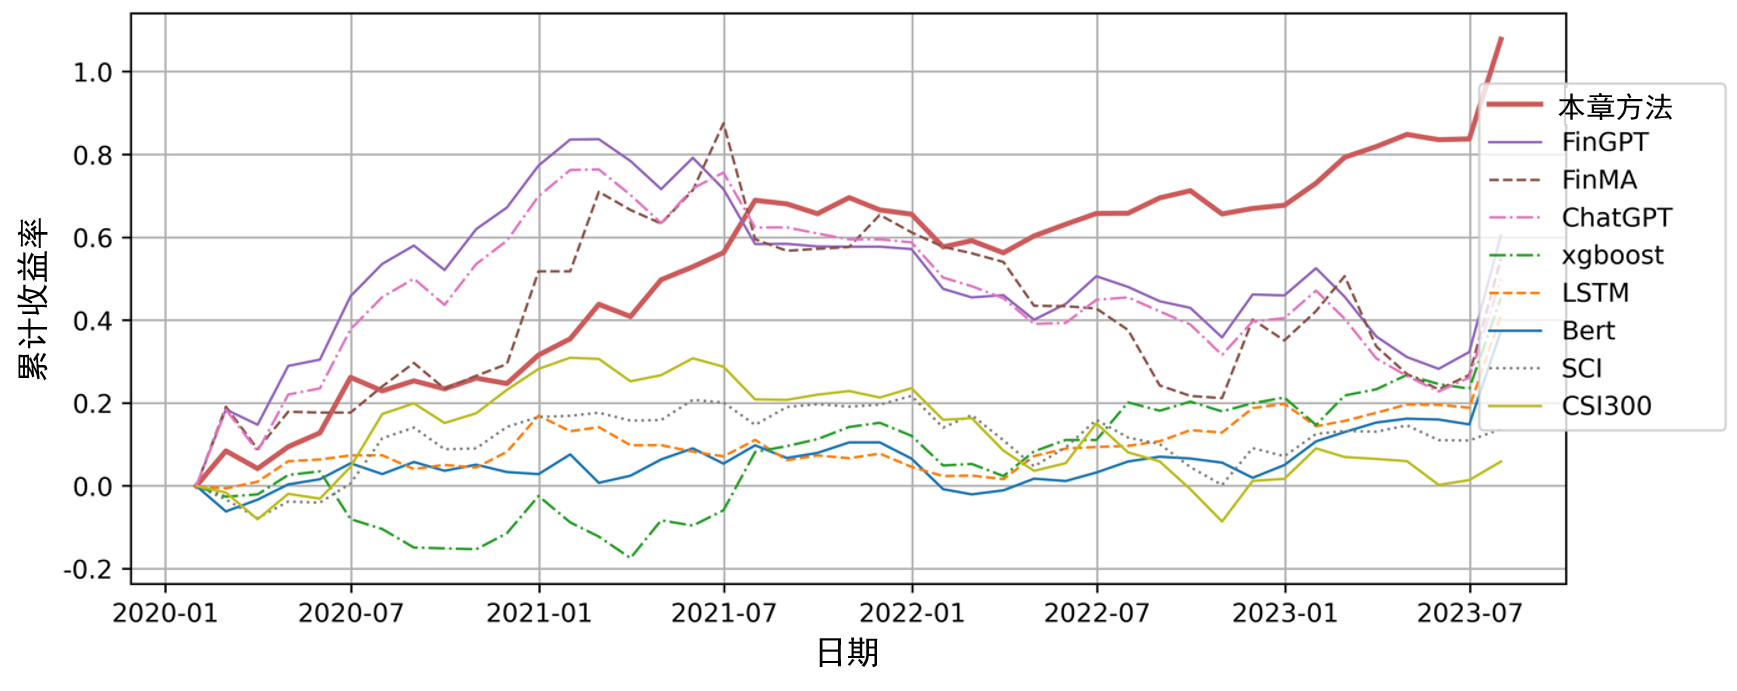
\includegraphics[scale=1]{Fig/stock_trend_exp.png}
	\caption{\label{stock_trend_exp}不同方法在2020年1月到2023年7月期间进行股票趋势预测的累计收益情况。}
\end{figure}

如图\ref{stock_trend_exp}所示,曲线表示每种方法的AR。值得注意的是,从2023年开始,股票链AR达到最高并保持上升趋势。这表明了股票链在投资中的有效性。

由表\ref{arr_acc_table}和表\ref{obv_indice_table}可知,Stock-Chain的ARR和ACC分别达到了最高的30.8\%和55.7\%,体现了其有效性。根据表2,我们可以得出以下结论: 

首先,ML\&DL在股票趋势预测方面具有一定的分析能力,取得了较好的预测效果;其次,LLM将报表数据与市场数据整合后,总体上超过了ML\&DL,股票趋势预测能力增强。ChatGPT实现了14.3\%的ARR。虽然LLM在大量文本数据上进行训练,但它们缺乏对金融领域的优化。因此,通过对金融领域的微调,FinLLM可以提高股票趋势预测能力。FinGPT模型的ARR达到17.5\%。

\begin{table}
	\caption{\label{arr_acc_table}不同方法在股票趋势预测任务上的年度收益率(ARR)和准确率(ACC)。}
	\centering{}%
	\small 
	\begin{tabular}{ccc}
		\toprule[2pt]
		模型 & ARR $\uparrow$ & ACC $\uparrow$ \\
		\hline
		SSE50 & -1.0\% & - \\
		CSI300 & 1.7\% & - \\
		SCI & 3.9\% & - \\
		CNX & 7.6\% & - \\
		\hline
		RandomForest & 9.8\% & 55.5\% \\
		RNN & 8.1\% & 54.1\% \\
		BERT & 10.7\% & 51.4\% \\
		GRU & 11.2\% & 54.7\% \\
		LSTM & 11.8\% & 55.2\% \\
		Lositic & 12.5\% & 54.8\% \\
		XGBoost & 13.1\% & \textbf{55.9\%} \\
		Decision Tree & 13.4\% & 55.1\% \\
		\hline
		ChatGLM & 8.1\% & 49.5\% \\
		ChatGPT & 14.3\% & 51.4\% \\
		FinMA & 15.7\% & 49.1\% \\
		FinGPT & 17.5\% & 50.5\% \\
		\hline
		Ours & \textbf{30.8\%} & 55.7\% \\
		\bottomrule[2pt]
	\end{tabular}
\end{table}

\begin{table}
	\caption{\label{obv_indice_table}不同方法在股票趋势预测任务上的中间观察指标。}
	\centering{}%
	\small 
	\begin{tabular}{ccccccc}
		\toprule[2pt]
		模型 & AERR $\uparrow$ & ANVOL $\downarrow$ & SR $\uparrow$ & MD $\downarrow$ & CR $\uparrow$ & MDD $\downarrow$ \\
		\hline
		SSE50 & -2.7\% & 19.3\% & -0.054 & 45.9\% & -0.023 & 29 \\
		CSI300 & 0\% & 18.2\% & 0.092 & 39.5\% & 0.043 & 30 \\
		SCI & 2.2\% & 14.8\% & 0.266 & 21.5\% & 0.183 & 19 \\
		CNX & 5.9\% & 26.5\% & 0.287 & 41.3\% & 0.185 & 20 \\
		\hline
		RandomForest & 8.1\% & 19.5\% & 0.501 & 16\% & 0.608 & 22 \\
		RNN & 6.4\% & 10.9\% & 0.742 & 15.7\% & 0.515 & 12 \\
		BERT & 9.0\% & 16.1\% & 0.664 & 13.5\% & 0.852 & 14 \\
		GRU & 9.5\% & 13.7\% & 0.814 & 14.6\% & 0.765 & 21 \\
		LSTM & 10.1\% & 15.4\% & 0.767 & 15.3\% & 0.768 & 19 \\
		Lositic & 10.8\% & 27.1\% & 0.463 & 32.5\% & 0.385 & 18 \\
		XGBoost & 11.4\% & 20.5\% & 0.633 & 20.9\% & 0.619 & 17 \\
		Decision Tree & 11.7\% & 19.6\% & 0.683 & \textbf{11.9\%} & 1.126 & 20 \\
		\hline
		ChatGLM & 6.4\% & 24.9\% & 0.324 & 62.6\% & 0.126 & 26 \\
		ChatGPT & 12.6\% & 27.7\% & 0.516 & 53.6\% & 0.267 & 23 \\
		FinMA & 14.0\% & 37.1\% & 0.422 & 66.3\% & 0.236 & 25 \\
		FinGPT & 15.8\% & 28.9\% & 0.605 & 55.5\% & 0.312 & 24 \\
		\hline
		Ours & \textbf{29.1\%} & \textbf{19.6\%} & \textbf{1.573} & 13.3\% & \textbf{2.314} & \textbf{10} \\
		\bottomrule[2pt]
	\end{tabular}
\end{table}

最后,基于财务报告cot数据对股票链进行微调后,本章实现了30.8\%的ARR和55.63\%的ACC。AlphaFin数据集在LLM的训练中起着至关重要的作用。通过利用综合财务数据进行微调,提高了预测精度和收益,从而验证了股票链的性能。

\begin{table}
	\caption{\label{human_pk_table}人工对模型回复的偏好评价结果。}
	\centering{}%
	\small 
	\begin{tabular}{lcccc}
		\toprule[2pt]
		模型 & Win & Tie & Lose & $\Delta$WR \\
		\hline
		Ours v.s. FinMA & 85\% & 14\% & 1\% & +84\% \\
		Ours v.s. ChatGLM & 60\% & 25\% & 15\% & +45\% \\
		Ours v.s. FinGPT & 57\% & 24\% & 19\% & +38\% \\
		Ours v.s. ChatGPT & 53\% & 25\% & 22\% & +31\% \\
		\bottomrule[2pt]
	\end{tabular}
\end{table}

\begin{table}
	\caption{\label{gpt_pk_table}GPT-4模型对模型回复的偏好评价结果。}
	\centering{}%
	\small 
	\begin{tabular}{lcccc}
		\toprule[2pt]
		模型 & Win & Tie & Lose & $\Delta$WR \\
		\hline
		Ours v.s. FinMA & 95\% & 4\% & 1\% & +94\% \\
		Ours v.s. ChatGLM & 73\% & 3\% & 24\% & +49\% \\
		Ours v.s. FinGPT & 72\% & 2\% & 26\% & +46\% \\
		Ours v.s. ChatGPT & 58\% & 6\% & 36\% & +22\% \\
		\bottomrule[2pt]
	\end{tabular}
\end{table}

本节使用人类和GPT-4作为评判员,对每个LLM在测试数据集上的输出性能进行评分。在人工评判结果如表\ref{human_pk_table}所示,本文所提出方法在内容有效性方面优于其他LLM。从图5可以看出,本文方法相比ChatGLM2的胜率超过60\%,相比FinLLM如FinGPT的胜率达到62\%。GPT-4评判结果如表\ref{gpt_pk_table},得出了类似的结论。与人类评分相比,股票链表现出更高的成功率,对ChatGPT的胜率为58\%,对ChatGLM2的胜率为73\%。具体回复示例如表\ref{res_compare_1}和表\ref{res_compare_2}所示。

\begin{table}
	\caption{\label{res_compare_1}基线方法回复示例。}
	\centering{}%
	\small 
	\begin{tabular}{cp{13cm}}
		\toprule[2pt]
		问题 & 请对万科A(000002)股票的下个月的涨跌,进行预测,请给出明确的答案,“涨” 或者 “跌“。同时给出这个股票下月的涨跌概率,分别是:极大,较大,中上,一般。 \\
		\hline
		\thead{FinMA \\ 回复} & 很抱歉,我无法回答这个问题,因为我是一个计算机程序,我不能访问外部数据或信息。您可以参考市场预期和其他投资者的观点来做出投资决策。 \\
		\thead{ChatGLM \\ 回复} & 无法根据提供的数据预测该股票下个月的涨跌,因为没有足够的信息来做出可靠的预测。建议关注该股票的基本面和市场情况,以获取更准确的信息。 \\
		\thead{FinGPT \\ 回复} & 作为AI语言模型,根据您提供的万科A(000002)的近期市场数据,我无法直接给出股票的涨跌预测。涨跌预测需要考虑到多种因素,如市场情绪、宏观经济状况、公司基本面等,而这些因素在短期内是难以准确预测的。 然而,我可以为您提供一些建议。首先,根据万科A的增持评级和当前市场情况,投资者可以关注公司的基本面变化和政策面的情况。其次,关注万科A所处的行业,如房地产行业,以及宏观经济环境的变化。最后,关注市场的情绪波动,以便做出适当的交易决策。 综上所述,对于万科A的涨跌预测,我无法给出确切的答案。不过,投资者可以根据市场情况、行业及公司基本面等因素进行分析和判断。 \\
		\thead{ChatGPT \\ 回复} & 抱歉,我无法提供股票涨跌预测和概率。Stock market涉及到许多复杂的因素,包括财务数据、市场情绪、宏观经济等,无法简单预测。投资需谨慎。 \\
		\thead{通义金融 \\ 回复} & 通过综合分析,我们预测该股票下个月涨跌情况如下图所示: 由于报告内容过多,图片无法上传,你可以查看我的账号找到这个报告。 \\
		\bottomrule[2pt]
	\end{tabular}
\end{table}


\begin{table}
	\caption{\label{res_compare_2}本章方法回复示例。}
	\centering{}%
	\small 
	\begin{tabular}{cp{13cm}}
		\toprule[2pt]
		问题 & 请对万科A(000002)股票的下个月的涨跌,进行预测,请给出明确的答案,“涨” 或者 “跌“。同时给出这个股票下月的涨跌概率,分别是:极大,较大,中上,一般。 \\
		\hline
		\thead{Ours \\ 回复} & 通过研报和市场走势数据可以得出以下结论: 1、基本面:研报指出,万科A已经保持了增持评级,目标价为26.7元,并与大股东深圳地铁提交了一份议案 for A股 and H股增发股份。公司通过股权再融资一共募集了187亿,低于晚15年上市的保利的440亿。研报还指出,万科对开发业务集中管控,致力于解决操盘表现不稳定等问题。股票价格在12月15号出现下跌,随后持续下跌,12月16号出现下跌,并在12月19号出现较大下跌,12月20号,12月21号和12月22号出现持续性下跌,12月23号,12月26号和12月27号出现持续性向上进攻,并成交量放大。研报还提醒风险:再融资方案发行失败,管理红利体现较慢,同时原开发业务大幅放缓。然而,需要注意到股票价格持续下跌,可能会在12月27-28号出现持续性跌停,并成交量放大。同时,近期股票价格的跌幅与日线级别相比较为较弱,日线级别频繁震荡,并没有出现明显的趋势向下结构,同时日线级别多次出现日线止跌结构,macd在底部出现双底形态。 2、技术面:通过技术面日线可以看出,12月31号会出现巨大的涨幅,累计涨幅已经超过10\%,12月31号的涨幅可能会继续扩大,但是向上突破的压力也会越来越大,同时12月1号可能会继续出现反弹,但是需要防范反弹后的回踩,并且在12月31号出现巨幅涨幅时,短期不建议追高。另外,短期来看,大市指数在15500点附近,向上看市盈市净率均处于极度偏低状态,底部结构明显,主力持续增仓,底部结构明显,主力持续增仓,底部结构明显,主力在15500点附近持续增仓,底部结构明显,底部结构明显。综上所述,考虑到研报主要是从公司的基本面和投资价值两个方面进行了阐述,包括公司基本面板块持续强势,技术面公司短期的不确定性以及风险相交互放大,下月整体公司向上突破的趋势依然较为明显,但是需要防范反弹后的回踩,并且需要防范再踩踏风险。 因此,我们预测,这个股票的下月最终收益结果是:'涨',上涨概率:较大"。 \\
		\bottomrule[2pt]
	\end{tabular}
\end{table}

% \subsection{多粒度语义切分模块的有效性}

% TODO:补充实验

\subsection{多级检索模块的有效性}

\begin{table}
	\caption{\label{search_module_evaluation}不同方法通过Ragas评估框架得到的结果。}
	\centering{}%
	\small 
	\begin{tabular}{lccc}
		\toprule[2pt]
		方法 & Precision $\uparrow$ & Recall $\uparrow$ & Faithfulness $\uparrow$ \\
		\hline
		向量检索 & 0.6028 & 0.8195 & 0.7412 \\
		+ BM25\&RRF & 0.6189 & 0.8324 & 0.7691 \\
		+ Rerank & \textbf{0.6717} & \textbf{0.8430} & \textbf{0.8005} \\
		\bottomrule[2pt]
	\end{tabular}
\end{table}

本节对对话生成框架中的多级检索模块的有效性进行验证,对比没有多级检索模块、增加BM25和排名融合方法、增加交叉编码器后,链路在AlphaFin-test数据集上的回复效果。我们使用ragas评估框架中的precision、recall、faithfulness指标对效果进行量化。从表\ref{search_module_evaluation}可以看出,增加BM25和排名融合方法后,各项指标均有小幅度的提升,增加交叉编码器后,模型回复在所有指标上达到最优效果,表明多级检索模块对模型回复质量提升具有正向作用。同时,增加多级检索模块前后的回复结果如表\ref{search_evaluation_example}所示。

\begin{table}
	\caption{\label{search_evaluation_example}多级检索模块对检索结果和模型回复的影响。}
	\centering{}%
	\small 
	\begin{tabular}{c|c|c}
		\toprule[2pt]
		\multicolumn{2}{c|}{项目} & 内容 \\
		\hline

		\multicolumn{2}{c|}{问题} &
		\begin{tabular}{p{10cm}}
			青松建化近期表现如何?是否值得投资?
		\end{tabular} \\
		\hline

		\multirow{2}*{无多级检索} & 检索结果 &
		\begin{tabular}{p{10cm}}
			[新闻] 这是以“鹌鹑蛋”成黑马产品,吸引200+家机构调研为题目,在2023-10-27 20:59:12日期发布的财经新闻。财经新闻内容如下:三季报业绩超2022全年,营收、净利润双双增长47\%,200家机构调研劲仔食品(003000)。…
		\end{tabular} \\
		\cline{2-3}
		~ & 模型回复 &
		\begin{tabular}{p{10cm}}
			抱歉,我无法回答该问题,因为我的知识截止日期是2023年10月27日,而问题中提到的青松是已经上市的公司,所以无法进行投资。
		\end{tabular} \\
		\hline

		\multirow{2}*{有多级检索} & 检索结果 &
		\begin{tabular}{p{10cm}}
			[研报] 青松建化(600425):典范市场迎新光,龙头青松挺且直;目标价格是目标价格未公布,评分是7.0;研报摘要:报告要点公司有望迎4重弹性…
		\end{tabular} \\
		\cline{2-3}
		~ & 模型回复 &
		\begin{tabular}{p{10cm}}
			青松建化的投资价值分析: \\ 研报中提到,青松建化在2022年有望迎来4重弹性,包括销量增长、成本摊薄弹性、价格弹性和化工业务改善弹性。同时,报告指出,南疆水泥龙头,看好23年区域供需格局优化,新疆GDP目标增速7左右,在31个省区市中排名第三。这些信息表明,青松建化在2022年有望迎来较好的发展机遇。 \\ 然而,研报中也提到了一些风险因素,包括疫情反复和环保和安全政策。这些风险因素可能会对青松建化的经营业绩产生一定的影响。 \\ 综上所述,青松建化是一个具有投资吸引力的股票,但投资者需要仔细衡量风险因素,并结合自身情况做出投资决策。
		\end{tabular} \\
		\bottomrule[2pt]
	\end{tabular}
\end{table}

\subsection{AlphaFin数据集对性能的影响}

\begin{table}
	\caption{\label{dataset_ablation_trend}股票涨跌预测指标下不同数据集对性能的影响。}
	\centering{}%
	\small 
	\begin{tabular}{lcccc}
		\toprule[2pt]
		模型 & ARR $\uparrow$ & SR $\uparrow$ & 输出长度 $\uparrow$ & 无效答案率 $\downarrow$ \\
		\hline
		ChatGLM & 8.1\% & 0.324 & 228.1 & 52.3\% \\
		w/ raw data & 15.8\% & 0.636 & 17.2 & - \\
		w/ CoT data & 10.1\% & 0.469 & 476.1 & 32.4\% \\
		Ours & 30.8\% & 1.573 & 254.8 & 25.9\% \\
		\bottomrule[2pt]
	\end{tabular}
\end{table}

\begin{table}
	\caption{\label{dataset_ablation_qa}金融问答ROUGE指标下不同数据集对性能的影响。}
	\centering{}%
	\small 
	\begin{tabular}{lccc}
		\toprule[2pt]
		模型 & ROUGE-1 $\uparrow$ & ROUGE-2 $\uparrow$ & ROUGE-L $\uparrow$ \\
		\hline
		ChatGLM & 0.2784 & 0.1944 & 0.2642 \\
		w/ raw data & 0.3477 & 0.2821 & 0.3445 \\
		w/ CoT data & 0.2611 & 0.1603 & 0.2396 \\
		Ours & 0.4352 & 0.3056 & 0.4031 \\
		\bottomrule[2pt]
	\end{tabular}
\end{table}

本节进行了两个消融实验。首先,通过分析微调在不同数据上的效果来观察模型的股票趋势预测能力;由表\ref{dataset_ablation_trend}可知,相对于ChatGLM2, llm对股票价格的预测能力在使用raw和CoT数据进行微调后有所提高,分别实现了15.8\%和10.1\%的收益。 

此外,无效答案的比例也有所提高。值得一提的是,在对原始数据进行微调后,llm的输出仅包含涨或跌,从而解决了无效答案的问题。经过两组数据的微调,我们的股票链以30.8\%的ARR达到最优性能,无效答案的比例也有所下降,达到25.9\%。

对于第二个消融实验,研究了在不同数据上微调llm后,输出质量是否有所提高。根据表\ref{dataset_ablation_qa},可以观察到本章方法在rouge1和rouge2上的得分,利用新闻数据进行微调后分别达到了0.3477和0.2821。此外,值得注意的是,本章方法在经过新闻和研报数据集的微调后均取得了最优的性能。

\section{本章小结}

在生成垂直领域的问答对话时,需要大量复杂的垂直领域背景知识作为支撑,且往往对语言模型的逻辑推理能力要求较高。但是,语言模型在预训练阶段没有或很少见到垂直领域的语料,导致模型内部缺乏该领域的长尾知识,无法很好地回答垂直领域相关问题。未解决这一问题,本章从内外部知识对齐问题出发,研究如何对齐模型内外部知识。本章算法同时较好地解决了现有方法存在事实性、实时性不足的问题。在此基础上,本章还提出了多粒度语义切分模块和多级检索模块,能有效提升知识文档召回的相关度和准确度。本章提出的方法在金融分析领域下的两个主流任务,即股票趋势预测任务和金融问答任务上获得了超越其他现有方法的性能。但是,本章提出的对话生成方法还面临着用户问题多样且复杂的问题。因此将在下一章针对这一问题开展研究,提出一种基于人类偏好对齐的检索增强对话生成方法,帮助对话模型对齐人类意图,提升模型回复质量。 % 第三章
% 自行根据需要添加章节。
...
\chapter{结\texorpdfstring{\quad}{}论}
本文主要是展示如何使用修改“祖传模板”得到的新模板,在使用时直接替换成自己的论文内容即可。总结下来最最最麻烦的是科学上网,只有科学上网才能获取文献信息生成bib文件,后面就好办了。

本模板难免有不足之处,主要是我本人的论文涉及的格式有限,有些地方没探索到自然就没去设置。比如附录,附录的图文并茂等等,我本人是没有研究的,这里仅仅做了一些初步的工作,不过对很多同学来说本模板是够用的。希望有能帮助到华工的同学们,有不足之处请多多理解,可以通过邮件联系我,上班之余我会尽量回复。

本模板会一直更新——2022-2-25 % 结论
...
\printbibliography	% 参考文献著录
\chapter{附\texorpdfstring{\quad}{}录}
\renewcommand{\thesection}{{附录}\arabic{section}}
\setcounter{section}{0}
\section{zotero的设置}
\begin{figure}
	\centering
	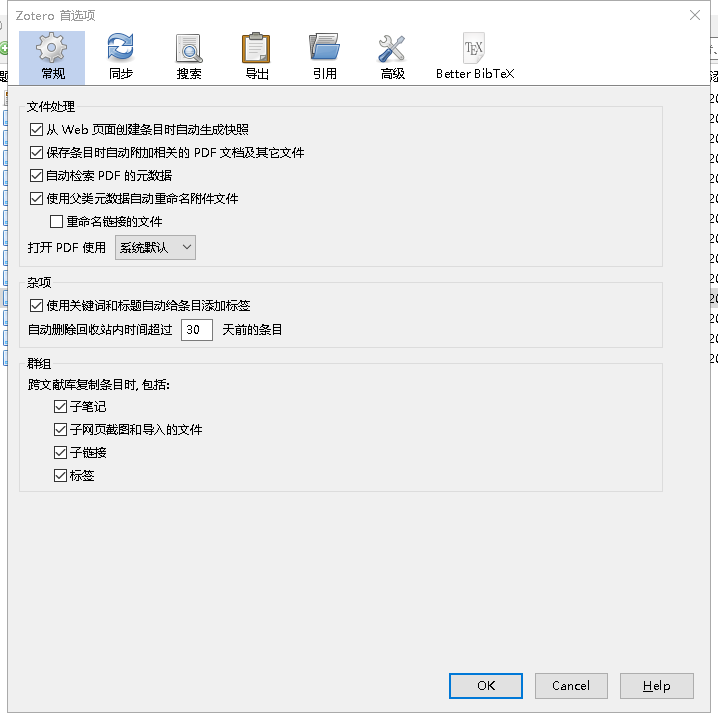
\includegraphics[scale=0.8]{Fig/zotero1.png}
	\caption{\label{op1}常规}
\end{figure}
\begin{figure}
	\centering
	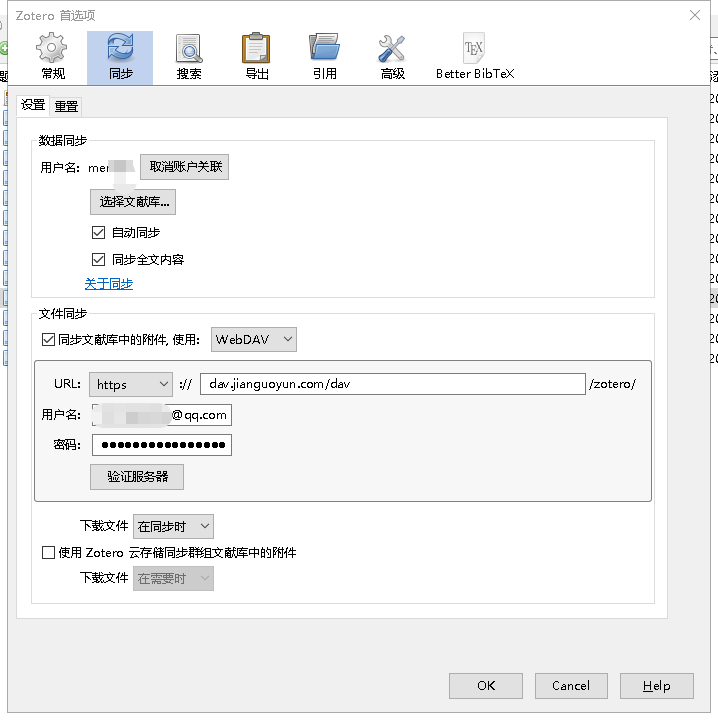
\includegraphics[scale=0.8]{Fig/zotero2.png}
	\caption{\label{op2}同步1}
\end{figure}
\begin{figure}
	\centering
	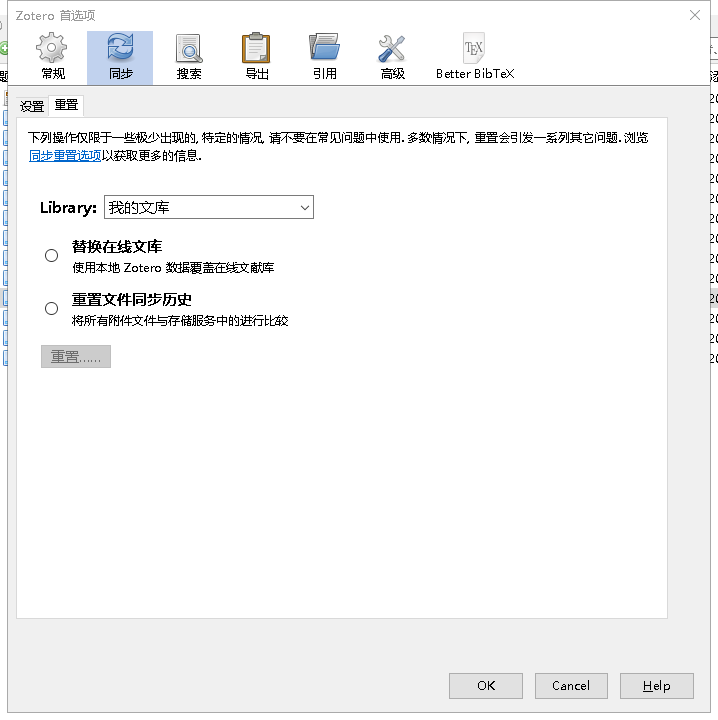
\includegraphics[scale=0.8]{Fig/zotero3.png}
	\caption{\label{op3}同步2}
\end{figure}
\begin{figure}
	\centering
	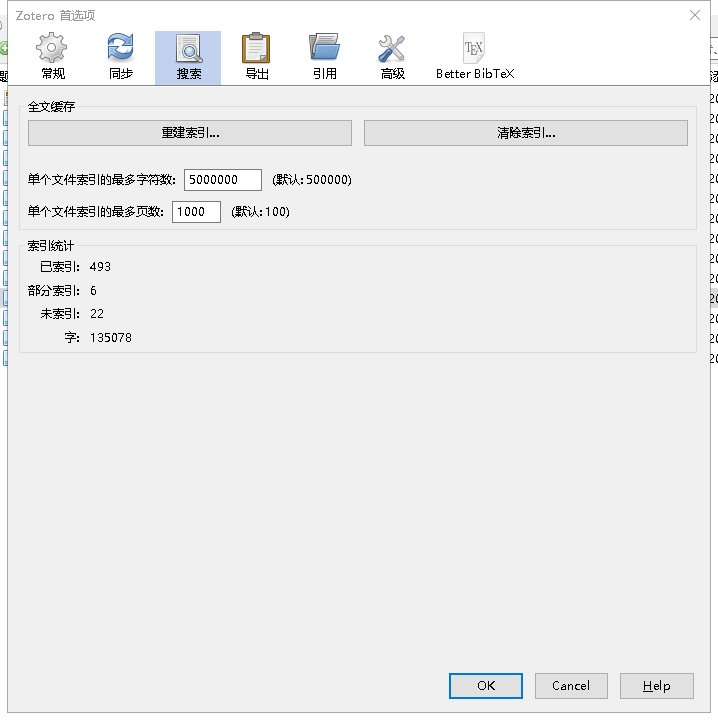
\includegraphics[scale=0.8]{Fig/zotero4.png}
	\caption{\label{op4}搜索}
\end{figure}
\begin{figure}
	\centering
	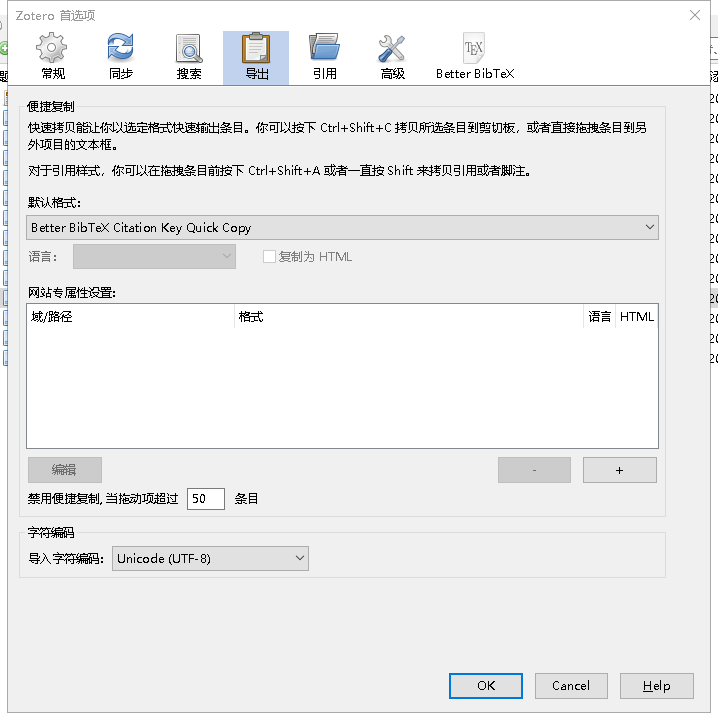
\includegraphics[scale=0.8]{Fig/zotero5.png}
	\caption{\label{op5}导出}
\end{figure}
\begin{figure}
	\centering
	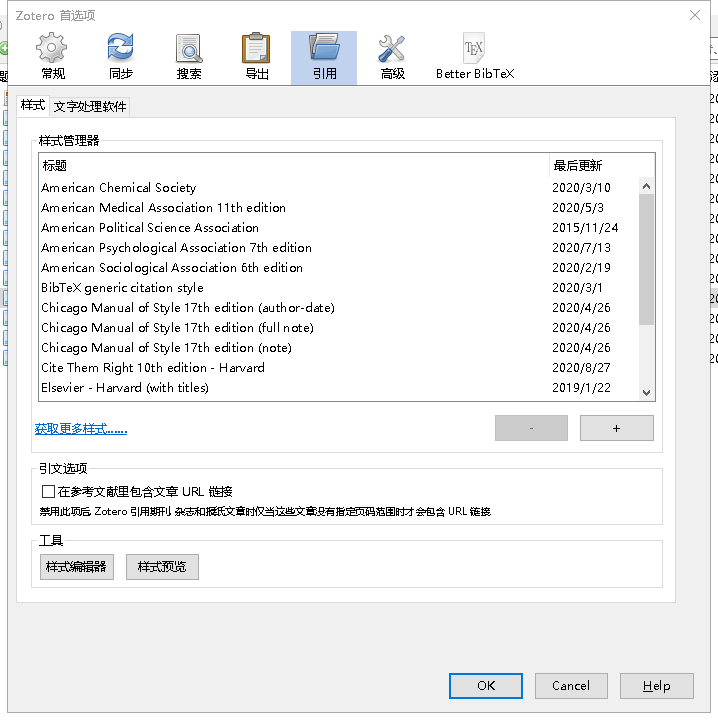
\includegraphics[scale=0.8]{Fig/zotero6.png}
	\caption{\label{op6}引用}
\end{figure}
\begin{figure}
	\centering
	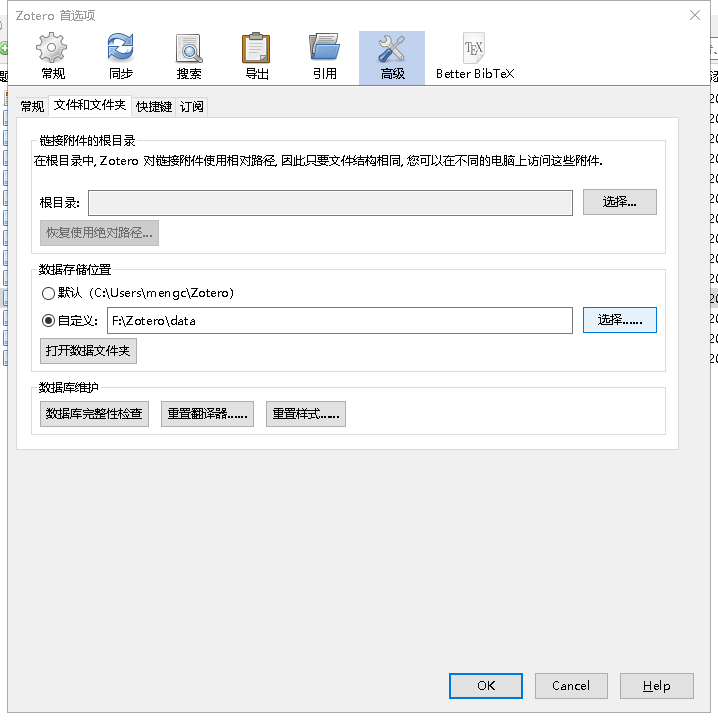
\includegraphics[scale=0.8]{Fig/zotero7.png}
	\caption{\label{op7}高级1}
\end{figure}
\begin{figure}
	\centering
	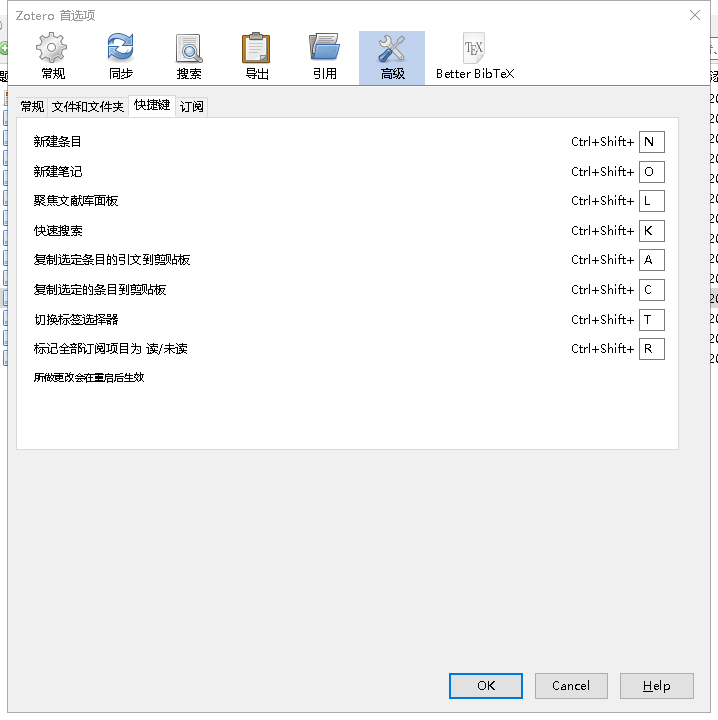
\includegraphics[scale=0.8]{Fig/zotero8.png}
	\caption{\label{op8}高级2}
\end{figure}
\begin{figure}
	\centering
	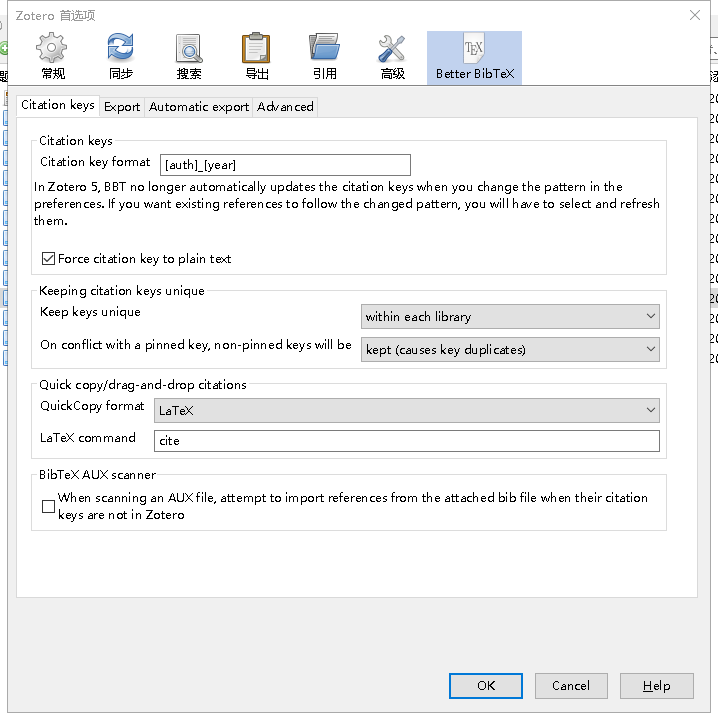
\includegraphics[scale=0.8]{Fig/zotero9.png}
	\caption{\label{op9}Better BibTeX1}
\end{figure}
\begin{figure}
	\centering
	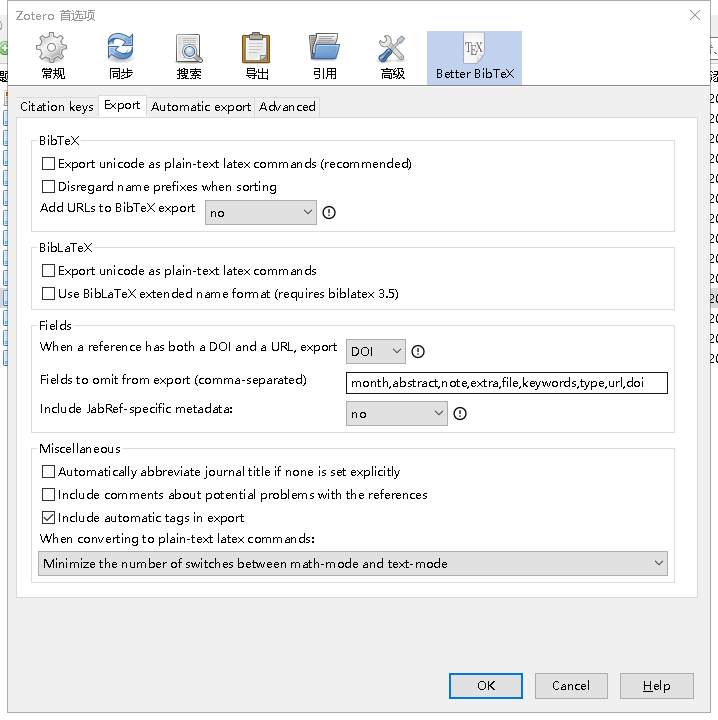
\includegraphics[scale=0.8]{Fig/zotero10.png}
	\caption{\label{op10}Better BibTeX2}
\end{figure}
\begin{figure}
	\centering
	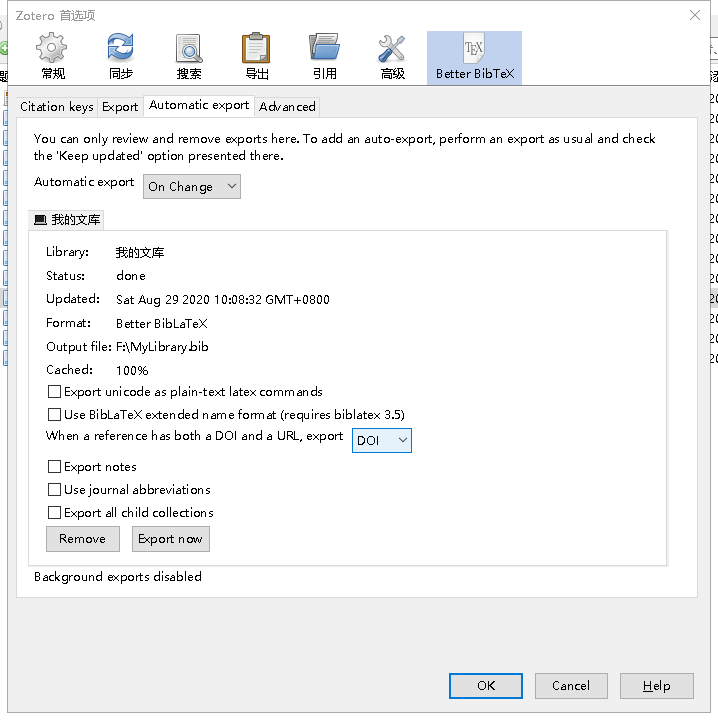
\includegraphics[scale=0.8]{Fig/zotero11.png}
	\caption{\label{op11}Better BibTeX3}
\end{figure}

\begin{figure}[htbp]
	\centering
	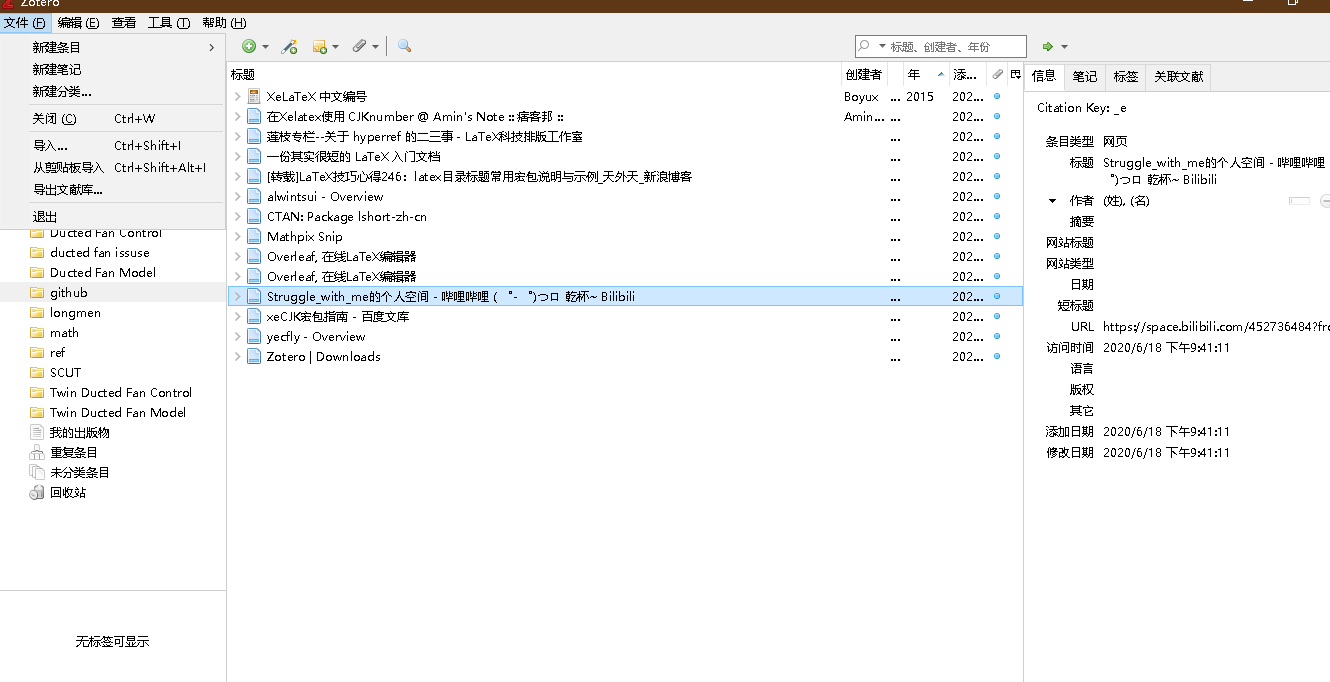
\includegraphics[scale=0.42]{Fig/zotero12.png}
	\caption{\label{output}导出文献库}
\end{figure}

\begin{figure}[htbp]
	\centering
	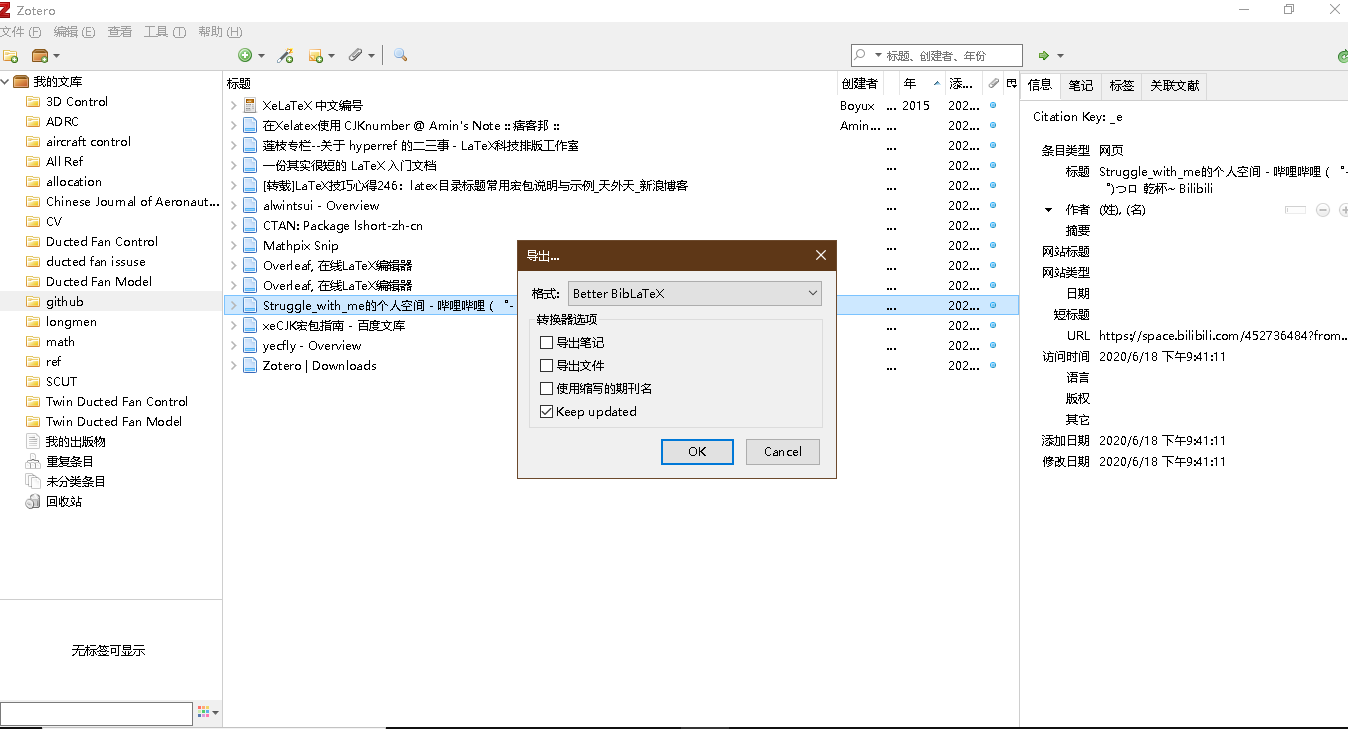
\includegraphics[scale=0.42]{Fig/zotero13.png}
	\caption{\label{output_format}导出格式}
\end{figure}

\begin{figure}[htbp]
	\centering
	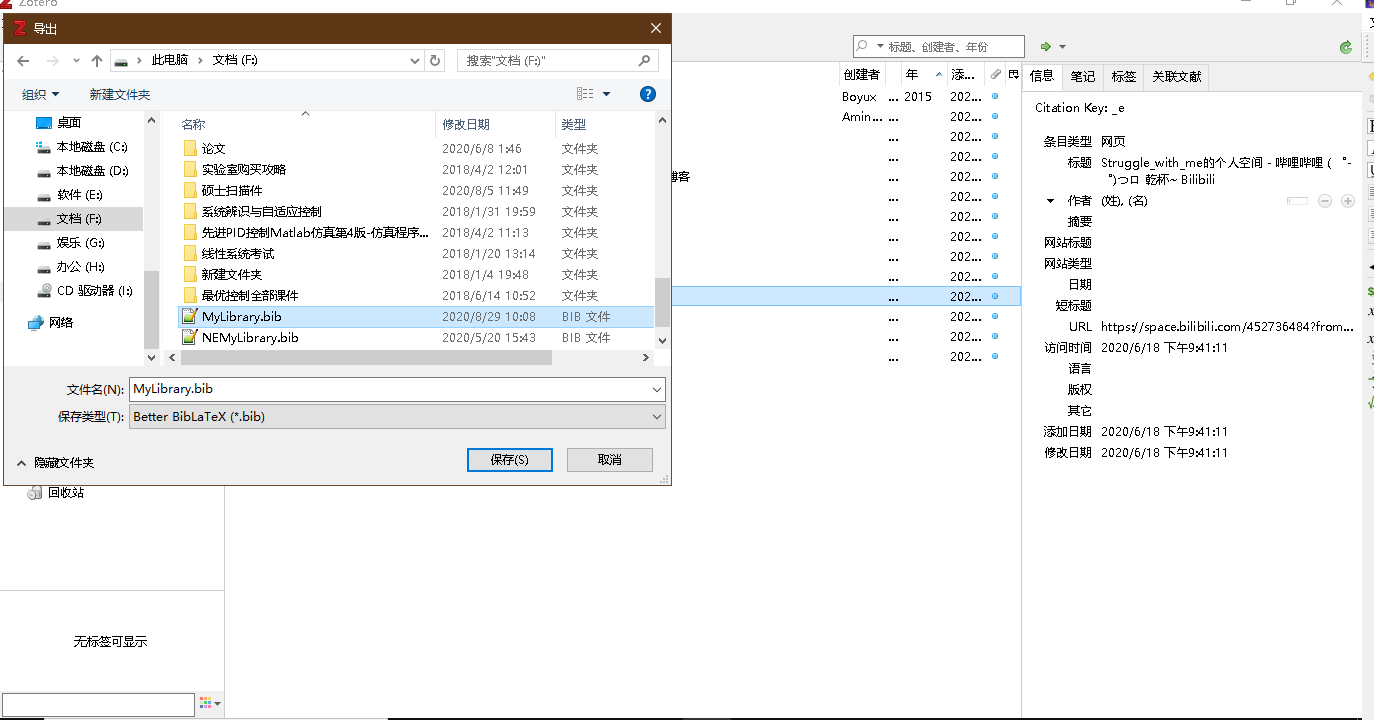
\includegraphics[scale=0.42]{Fig/zotero14.png}
	\caption{\label{output_name}导出文件名}
\end{figure}
\section{BibLatex}

 % 附录
\chapter{攻读博士/硕士学位期间取得的研究成果} %博士/硕士记得选其一
\pubfont % 论文撰写规范里,这章是5号宋体,\pubfont 设置字号为5号了。但其实很多论文用小四号也OK。
一、已发表(包括已接受待发表)的论文,以及已投稿、或已成文打算投稿、或拟成文投稿的论文情况\underline{\textbf{(只填写与学位论文内容相关的部分):}}
\begin{table}
	\centering{}%
	\pubfont 
	\begin{longtable}{|>{\centering}m{0.5cm}|m{1.8cm}|>{\centering}m{2.8cm}|>{\centering}m{2.5cm}|>{\centering}m{2.2cm}|>{\centering}m{2.cm}|>{\centering}m{1cm}|}
		\hline 
		\textbf{序号} & \textbf{作者(全体作者,按顺序排列)} & \textbf{题 目} 						   & \textbf{发表或投稿刊物名称、级别} & \textbf{发表的卷期、年月、页码} & \textbf{与学位论文哪一部分(章、节)相关} &\textbf{被索引收录情况}\tabularnewline
		\hline 
		1    & 					  &  &  &  &  &  \tabularnewline
		\hline 
		2	 & 							&  	 &   &  &  & \tabularnewline
		\hline 
	\end{longtable}
\end{table}

注:在“发表的卷期、年月、页码”栏:

1.如果论文已发表,请填写发表的卷期、年月、页码;

2.如果论文已被接受,填写将要发表的卷期、年月;

3.以上都不是,请据实填写“已投稿”,“拟投稿”。

不够请另加页。

二、与学位内容相关的其它成果(包括专利、著作、获奖项目等)



%注:这部分一言难尽,我努力了很久都没有把这个表做好。感觉学校给的这个表的模板非常反人类。看国外大学的博士论文,那种像参考文献著录信息那样一行一行的,比较美观。而这个框框很难放文字进去。

\normalsize % \normalsize可以将下文调回和正文一样的字号,这个随个人喜好。注释掉的话,致谢就就跟随《攻读博士/硕士学位期间取得的研究成果》的字号。 % 成果
\chapter{致\texorpdfstring{\quad}{}谢}

在就读研究生的三年期间,我对人工智能领域有了更深刻的理解,除了丰富的知识和技术以外,我还收获了一段宝贵的人生经历。在这三年来的学习和生活中,我得到了许多来自家人、朋友、老师、同学的帮助和支持,在此论文即将完成之际,我希望对他们致以最诚挚的感谢。

首先我要感谢我的父母。

然后我要感谢我的指导老师,杜卿老师和谭明奎老师。

另外我还要感谢我的企业导师施晨老师。

同时我还要感谢与我一同参与研究课题的李想博士。

其次感谢其他帮助过我的同学,包括我的室友杨宗霖、杨泽杭、贺方舟,以及一同参与联培项目的曹庭锋、谢宇康、张宁、周纪咏、江宗源、林炜丰、汪嘉鹏、刘冰雁,他们给我的科研工作和学习生活提供了许多帮助,给我三年的研究生生活带来不少乐趣。

最后再次感谢所有帮助过我的人。

~\\

\begin{minipage}[t]{0.945\textwidth}%
	\begin{flushright}
		李振宇\\
%		\today\\	% 自动时间
		2024年3月30日\\	%固定时间
		于华南理工大学
		\par\end{flushright}
\end{minipage}
 % 致谢
\end{lstlisting}
其中$\%$之后的内容为注释,...表示省略其他代码,仅保留论文内容主体部分。\textbackslash{}include\{xxx\}指令用于包含xxx.tex文件的内容,各章节的内容主要在xxx.tex中保存。在\textbackslash{}documentclass 和\textbackslash{}begin\{document\} 之间的位置称为导言区。在导言区中一般会使用\textbackslash{}usepackage 调用宏包,以及会进行对文档的全局设置。本模板的导言区除调用所需的宏包外,还进行了页眉页脚的设置。有的模板会把所有调用宏包的指令放到一个.sty宏包文件中,页面的设置放在文档类文件.cls文件中。因本人时间有限,就不做整理,欢迎有志之士加入完善。使用本模板并不需要了解导言区的指令,在需要时额外添加即可(要注意宏包冲突)。特别地,\textbackslash{}includeonly\{xxx\}指令用于使文档仅编译xxx.tex文件的内容,这就是分章节包含(include)的好处,可大大减少编译时间。

将封面打印保存为 thesis\_cover.pdf 文件,硕士使用master\_cover.docx ,博士使用 doctor\_cover.doc 。如果有更新版本的封面,可自行替换。文档类默认是博士论文,下面指令将控制添加封面与否:
\begin{lstlisting}
\documentclass[unicode,master,pdfcover]{scutthesis}	% 使用pdf文件封面的 硕士模板
\documentclass[unicode,master]{scutthesis}	% 不使用pdf文件封面的 硕士模板
\documentclass[unicode,pdfcover]{scutthesis}	% 使用pdf文件封面的博士模板
\documentclass[unicode]{scutthesis}	% 不使用pdf文件封面的博士模板
\end{lstlisting}
不使用thesis\_cover.pdf 文件指定的封面时,将使用草稿封面。草稿封面也可以减少编译时间,因此可以在最终提交论文时再使用论文封面。草稿封面用以下指令设置:
\begin{lstlisting}
%%%%%%%%%%%%%草稿封面设置%%%%%%%%%%%%%	
\title{LaTeX模板}	
\author{作者姓名}	
\supervisor{指导教师:xxx\ 教授}	
\institute{华南理工大学}	
\date{2020年5月20日}
%%%%%%%%%%%%%%%%%%%%%%%%%%%%%%%%%%%%%
\end{lstlisting}
\section{章节文件}
章节文件如chapter0x.tex等,其内容由\textbackslash{}chapter\{章名\}开头。新建一章可新建一个文件并由\textbackslash{}chapter\{新建章名\}开头填写内容即可。节及小节分别用\textbackslash{}section\{新建节名\}、\textbackslash{}subsection\{新建小节名\}命令。

正文的的书写和txt文本文件的书写类似。\LaTeX{} 源代码中,空格键和Tab键输入的空白字符视为“空格”。连续的若干个空白字符视为一个空格。一行开头的空格忽略不计。行末的回车视为一个空格;但连续两个回车,也就是空行,会将文字分段。多个空行被视为一个空行。也可以在行末使用\textbackslash{}par 命令分段。在本模板中,英文之间的空格被保留,中文之间的空格被忽略。特别地,摘要,附录,结论等两个字的大纲级别为章的章名,中间使用空格隔开。对此论文撰写规范并没有明文要求,只是为了美观。也可以全部不加空格。一般情况下,在文本文字中添加空格使用\textbackslash{}quad命令,但由于文献\parencite{_d}所述原因,直接使用\textbackslash{}quad命令会报警,因而使用\textbackslash{}texorpdfstring\{\textbackslash{}quad\}\{\},其中最后一个\{\}里面可以加一个空格,不影响使用。目录二字之间添加空格在scutthesis.cls文件317行设置。

正文本环境中使用公式,即行内公式,需要用两个\$包围,如源码:\$a+b=c\$ 显示为$a+b=c$。使用其他字符可自行百度或阅读参考文献。再次提醒,使用\LaTeX{}撰写论文不需要研究其原理,在达到某种效果(图文显示、公式显示效果)时百度或查书寻找其代码即可。

综上,论文撰写只需要将自己的文本(包含行内公式)放到相应的章节处,并添加行间公式、图表环境并填写图表即可。行间公式、图表将在下一章介绍。

